\documentclass[11pt]{article}
\usepackage[margin=2.5cm]{geometry}
\usepackage{amsmath}\usepackage{amssymb}\usepackage{graphicx}
\usepackage{booktabs}\usepackage{hyperref}
\graphicspath{{../../plots/emulator_tier3/}}
\newcommand{\Mpch}{\,h^{-1}\,\mathrm{Mpc}}
\newcommand{\code}[1]{\texttt{#1}}
\title{The Tier-3 ASTRA MLP emulator --- design, floor investigation, and inference prototype}
\author{ASTRA clustering project}\date{June 2026}
\begin{document}\maketitle

\begin{abstract}
This note specifies the first MLP emulator built on the Tier-3 pilot
(\code{data/fullbox\_tier3/}: 10 cosmologies $\times$ 50 HODs, all complete). It
fixes the emulator \emph{inputs}, the \emph{target} data vector (prioritising the
void/knot environments from the randoms, then the data, in monopole and
quadrupole), the \emph{cached dataset} that decouples slow disk reads from fast
retraining, the \emph{train/validation/test split} (leave-one-cosmology-out, not
a random split), the \emph{architecture}, and the \emph{diagnostic plots}. It is
the companion to \code{tier3\_emulator\_note.tex} (which sets the campaign
strategy); this note is the operational recipe the code implements.
\end{abstract}

\section{Inputs (20-D)}
The emulator maps $\theta = (\theta_{\rm cosmo},\theta_{\rm HOD}) \mapsto
\xi(s)$. The Tier-3 block \code{c130}--\code{c181} varies the broader
$w_0w_a$CDM$+$ set, so the cosmology input is \textbf{8 varying parameters}
(read from \code{data/abacus\_cosmologies\_params.csv}):
\[
\omega_b,\ \omega_{\rm cdm},\ h,\ n_s,\ \alpha_s,\ N_{\rm ur},\ w_0,\ w_a .
\]
($A_s$ and $\omega_{\rm ncdm}$ are fixed across the block; $\sigma_8$ is a
derived quantity and is kept as a label, not an input, to avoid collinearity.)
The HOD input is the \textbf{12 yuan23 parameters} already used throughout the
project: \code{LOGM\_CUT, LOGM1, SIGMA, ALPHA, KAPPA, ALPHA\_C, ALPHA\_S, S,
ACENT, ASAT, BCENT, BSAT}. Total input dimension \textbf{20}. All inputs are
standardised (zero mean, unit variance over the training set).

\section{Targets}
The science priority is the \textbf{extreme environments} --- voids (Q1) and
knots (Q4) --- \textbf{mostly from the randoms}, then from the data, in both
multipoles. The primary target legs are therefore
\[
\{\code{rand\_q1},\ \code{rand\_q4},\ \code{cross\_full\_rand\_q1},\ \code{cross\_full\_rand\_q4}\}
\]
followed by the data twins
$\{\code{data\_q1},\code{data\_q4},\code{cross\_full\_data\_q1},\code{cross\_full\_data\_q4}\}$,
each in $\ell=0$ and $\ell=2$. The current pilot multipoles are stored on the
coarse 15-bin $0$--$150\Mpch$ grid ($\sim 10\Mpch$ bins); the fine small-scale
binning the strategy note calls for would require a pipeline re-run and is
deferred. We train on the bins on disk and report accuracy as a function of a
scale cut $s_{\rm cut}$ so the small-scale ($s<40\Mpch$) payoff region is read
off directly.

\section{Cached dataset --- the key to cheap retraining}
We will retrain many times (different target subsets, architectures,
PCA truncations, loss weights). Re-globbing $\sim$1000 run directories each time
is wasteful, so a one-shot builder
(\code{scripts/build\_emulator\_dataset.py}) writes a single compact archive
\code{data/emulator\_tier3/dataset.npz} holding the \emph{full} stem set --- all
17 stems $\times\,2$ multipoles $\times\,15$ bins (510-D) --- even though the
first model trains on the void/knot subset. Arrays:
\begin{itemize}
\item \code{X\_cosmo} $(N,8)$, \code{X\_hod} $(N,12)$ --- standardisable inputs;
\item \code{Y} $(N,510)$ --- concatenated $[\xi_0,\xi_2]$ over stems;
\item \code{Ynoise} $(N,510)$ --- per-bin ASTRA-iteration scatter (\code{xi*\_std});
\item \code{s} (15,), \code{stem\_labels}, \code{ell\_labels}, \code{bin\_index} --- block bookkeeping;
\item \code{cosmo\_id}, \code{hod\_id}, \code{sigma8} --- per-row metadata for grouping/plots.
\end{itemize}
Target selection at train time is a column mask over \code{Y}; no disk re-read.
The same builder writes \code{dataset\_anchor.npz} from the 450 Fisher-grid runs
(\code{data/fullbox/}, cosmologies \code{c000,c100--c105,c112,c113}), which are
\emph{not} in the training block and serve as an independent generalisation
anchor in the LCDM neighbourhood.

\section{Train / validation / test split}
The decisive structural fact: there are only \textbf{10 cosmologies} but 500
runs. A random split over runs would place HODs of the same cosmology in both
train and test, leaking the (sparse, hard) cosmology axis and giving an
optimistic score. In deployment the emulator predicts at \emph{new}
cosmologies, so the split is made \textbf{along the cosmology axis}:
\begin{itemize}
\item \textbf{Headline: 10-fold leave-one-cosmology-out (LOCO).} Each fold trains
  on 9 cosmologies (450 runs) and tests on the held-out one (50 runs); rotating
  over folds tests every cosmology. This is the go/no-go metric.
\item \textbf{Inner validation:} within each fold's 9 training cosmologies,
  $\sim$15\% of the HODs (drawn across all 9, fixed seed) are held out for
  early-stopping and hyperparameter choices.
\item \textbf{Per-fold fractions} $\approx$ 76\% train / 14\% validation / 10\%
  test, partitioned by cosmology --- \emph{not} a random 70/15/15 over runs.
\item \textbf{External anchor:} the 450 Fisher-grid runs, never trained on, give
  a second test set in the dense LCDM region we ultimately care about.
\end{itemize}
LOCO is chosen over a fixed permanent holdout because 10 cosmologies is too few
to also sacrifice a standalone test block.

\section{Architecture}
SUNBIRD-style feed-forward MLP in \code{torch} (2.10, CUDA available):
\begin{itemize}
\item Input 20-D (standardised) $\to$ 3--4 hidden layers (256--512 units, SiLU)
  $\to$ output;
\item \textbf{Output via PCA} ($\sim$10--20 components on the standardised target
  vector) for a compact, decorrelated regression target;
\item \textbf{Noise-weighted MSE} loss, weight $1/\sigma_{\rm noise}^2$ per bin,
  for the pilot. (The covariance-weighted loss that matches the inference metric
  is the eventual goal, but the covariance is the known weak point of Tier-3, so
  we start diagonal.)
\item \textbf{Ensemble} of $\sim$5 independently-seeded MLPs for the emulator
  uncertainty (used in the pull/calibration diagnostic);
\item Adam, early stopping on the inner validation loss.
\end{itemize}

\section{Diagnostic plots}
Acceptance is judged per $s$-bin against two yardsticks already used at Tier-2:
the \textbf{ASTRA noise floor} (mean per-iteration $\xi_{\rm std}$, which no
emulator should be expected to beat) and the \textbf{signal spread} (std of the
training vectors, i.e.\ what there is to learn). A good emulator has
LOCO~RMS~$\sim$~noise floor and $\ll$~spread, especially at $s<40\Mpch$. Plots:
\begin{enumerate}
\item \textbf{Learning curves} --- train/validation loss vs epoch, per fold (overfit check).
\item \textbf{LOCO prediction vs truth} --- $s^2\xi$ for void/knot, data \& random,
  $\ell=0,2$, on the held-out cosmology.
\item \textbf{Error vs yardstick} --- per-bin LOCO RMS against noise floor and
  signal spread vs $s$, zoomed to $s<40\Mpch$ (the acceptance plot).
\item \textbf{Pull histograms} --- $(\hat\xi-\xi)/\sigma_{\rm ens}$ should be
  $\mathcal N(0,1)$ (ensemble-uncertainty calibration).
\item \textbf{Accuracy vs scale cut} --- RMS/noise integrated for $s<s_{\rm cut}$,
  directly answering ``sub-noise at $s<40$''.
\item \textbf{Fractional-error heatmap} --- (stem $\times\,\ell$) vs $s$-bin,
  colour $=$ median $|$frac.\ error$|$; an at-a-glance map (expect random
  quadrupoles weakest, per prior findings).
\item \textbf{External-anchor prediction vs truth} --- the same curves on the 9
  Fisher cosmologies.
\end{enumerate}

\section{Caveats}
Ten cosmologies over an 8-D cosmology input is thin: a poor LOCO result means
``need the full \code{c130}--\code{c181}$\times$120 campaign,'' not ``ASTRA
fails.'' The coarse 15-bin grid limits the very small-scale resolution that
carries most of the Fisher signal. The HOD response is assumed smooth and the
ASTRA-iteration noise (3 iterations in the pilot) sets a floor the emulator
cannot cross. These are the questions the diagnostics are designed to expose.

%======================================================================
\section{Results I: the floor investigation}
The pilot was run and the diagnostics above executed. The headline question
``can a monopole+quadrupole emulator reach inference-grade accuracy?'' decomposed,
through a sequence of cheap tests, into a clear and ultimately encouraging picture.
All ``$\times$CV'' numbers are ratios of the held-out RMS to the cosmic-variance
standard deviation at the $2\Mpch$\,Gpc box volume (see the \emph{CV correction}
subsection below for an important denominator fix).

\subsection{The pilot is extrapolation-limited, not broken}
Leave-one-cosmology-out training gives physical predictions and 7/10 folds beat the
mean, but the held-out error is large and \emph{varies enormously by cosmology}:
hull-centre cosmologies are predicted well, hull-edge ones badly. The learning curve
versus the number of training cosmologies (Fig.~\ref{fig:lc}) is essentially flat
across the 2--9 cosmologies the pilot can probe --- but those ten cosmologies are
spread every fifth point over the $w_0w_a$CDM hull, so this test cannot probe the
\emph{density} the full campaign would add. The conclusion is that the pilot is
\textbf{cosmology-extrapolation limited}: the cosmology axis is too sparsely sampled,
not that the method fails.

\begin{figure}[h]\centering
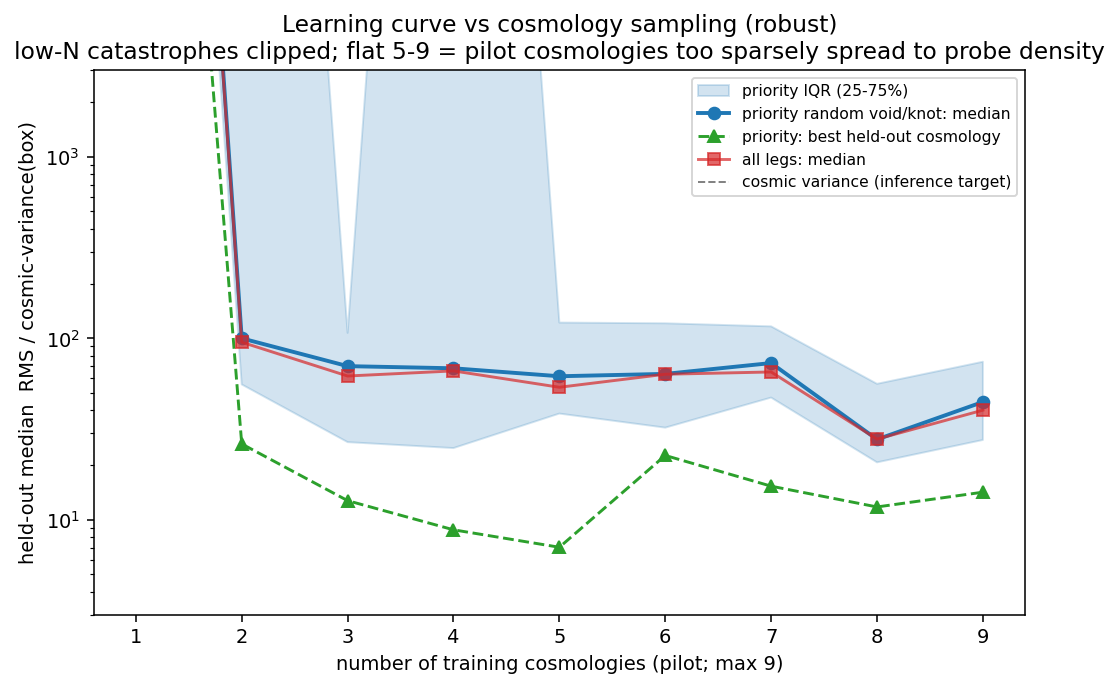
\includegraphics[width=0.62\textwidth]{mlp_learning_curve_vs_ncosmo.png}
\caption{Held-out error versus number of training cosmologies (robust median over
random subsets; RMS/spread panel is CV-estimate-noise-free). Flat across 2--9
cosmologies: at the pilot's sparse spacing, adding points does not shrink the
inter-cosmology gaps. The campaign changes the \emph{density}, which this proxy
cannot see.}
\label{fig:lc}
\end{figure}

\subsection{Ruling out the suspects}
A within-cosmology test (5-fold over each cosmology's HODs, \emph{zero} cosmology
extrapolation) isolates a second, smaller floor (Fig.~\ref{fig:within}). We then
eliminated its candidate causes one by one:
\begin{itemize}
\item \textbf{HOD sample size --- ruled out.} The within-cosmology floor plateaus by
  $\sim$30 training HODs and does not improve out to 70 (we ran \code{c000} to 100
  HODs to check; Fig.~\ref{fig:hodcurve}).
\item \textbf{Model class / loss / representation --- ruled out.} A bake-off of the
  MLP against a PCA$+$GP (covariance-weighted, amplitude-factored residual target)
  and a PCA$+$Ridge all tie (Fig.~\ref{fig:bakeoff}).
\item \textbf{Iteration noise --- ruled out} earlier (emulator error $\gg$ the ASTRA
  per-iteration scatter).
\item \textbf{Binning --- ruled out.} A zero-compute coarsening proxy (rebin the
  existing data to 3--15 bins) shows the modelling-quality metric (RMS/spread,
  immune to CV-estimate noise) is flat with resolution (Fig.~\ref{fig:binproxy});
  the apparent gain toward finer bins in RMS/CV is a noisy-denominator artifact.
  Finer binning is therefore \emph{not} a strong lever.
\end{itemize}

\begin{figure}[h]\centering
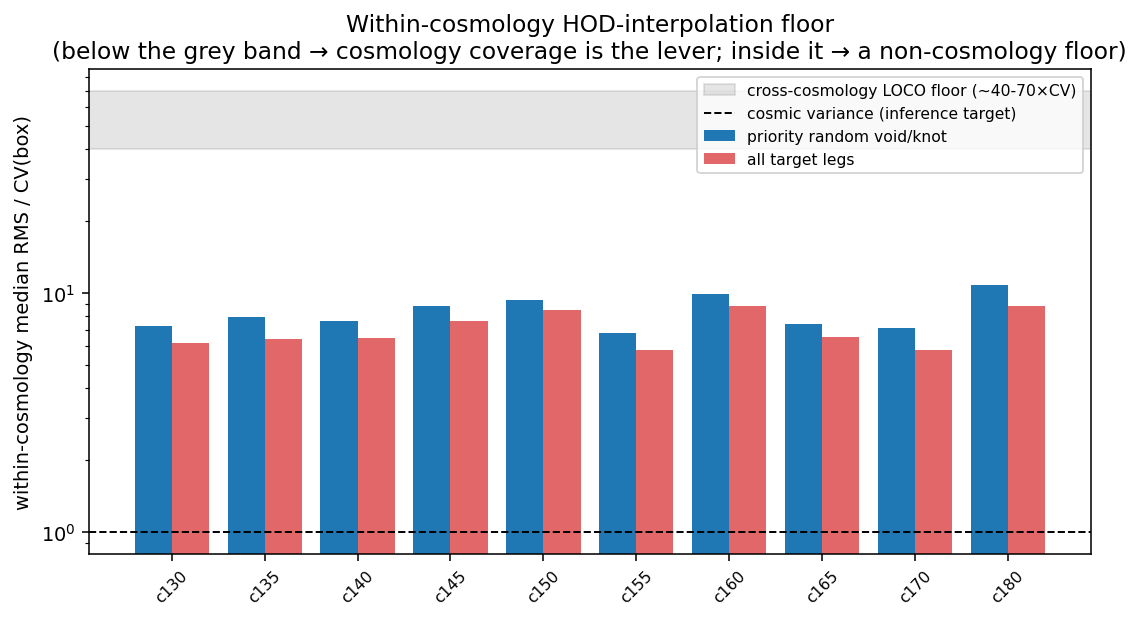
\includegraphics[width=0.74\textwidth]{mlp_within_cosmo_floor.png}
\caption{Within-cosmology HOD-interpolation floor per cosmology (zero cosmology
extrapolation). A uniform residual floor remains even with no extrapolation; its
cause is isolated in the following tests.}
\label{fig:within}
\end{figure}

\begin{figure}[h]\centering
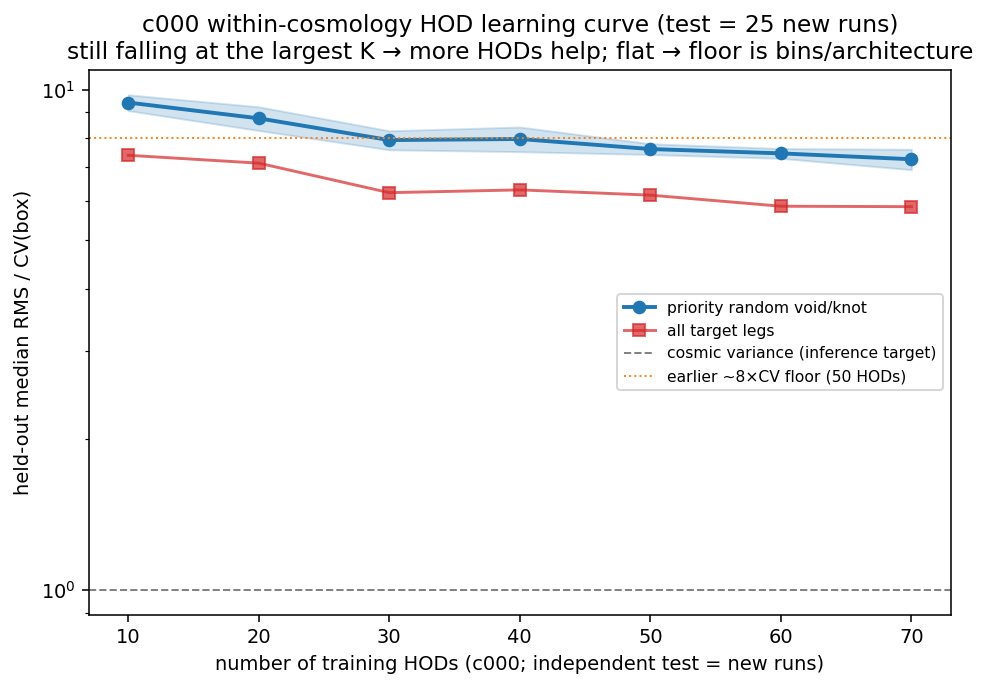
\includegraphics[width=0.49\textwidth]{mlp_c000_hod_curve.png}\hfill
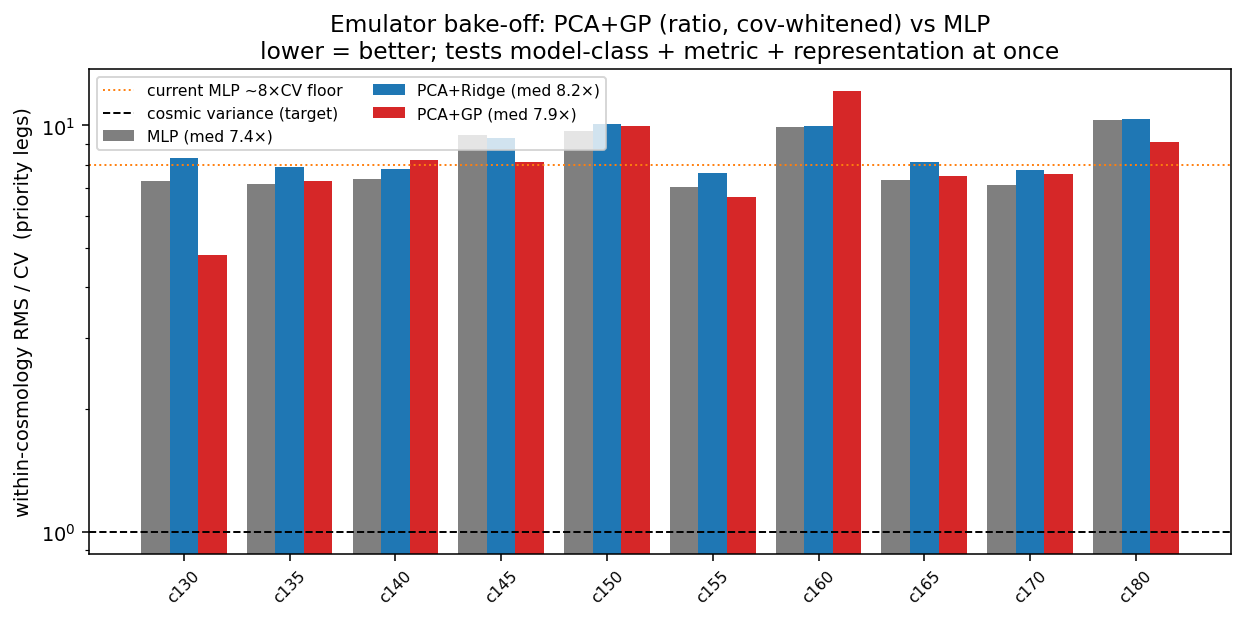
\includegraphics[width=0.49\textwidth]{emulator_bakeoff.png}
\caption{\emph{Left:} \code{c000} held-out error vs.\ number of training HODs
(100 HODs available): plateaus by $\sim$30 --- HOD count is not the limiter.
\emph{Right:} model bake-off, within-cosmology floor per cosmology --- MLP,
PCA$+$Ridge and PCA$+$GP tie, so model/loss/representation is not the limiter.}
\label{fig:hodcurve}\label{fig:bakeoff}
\end{figure}

\begin{figure}[h]\centering
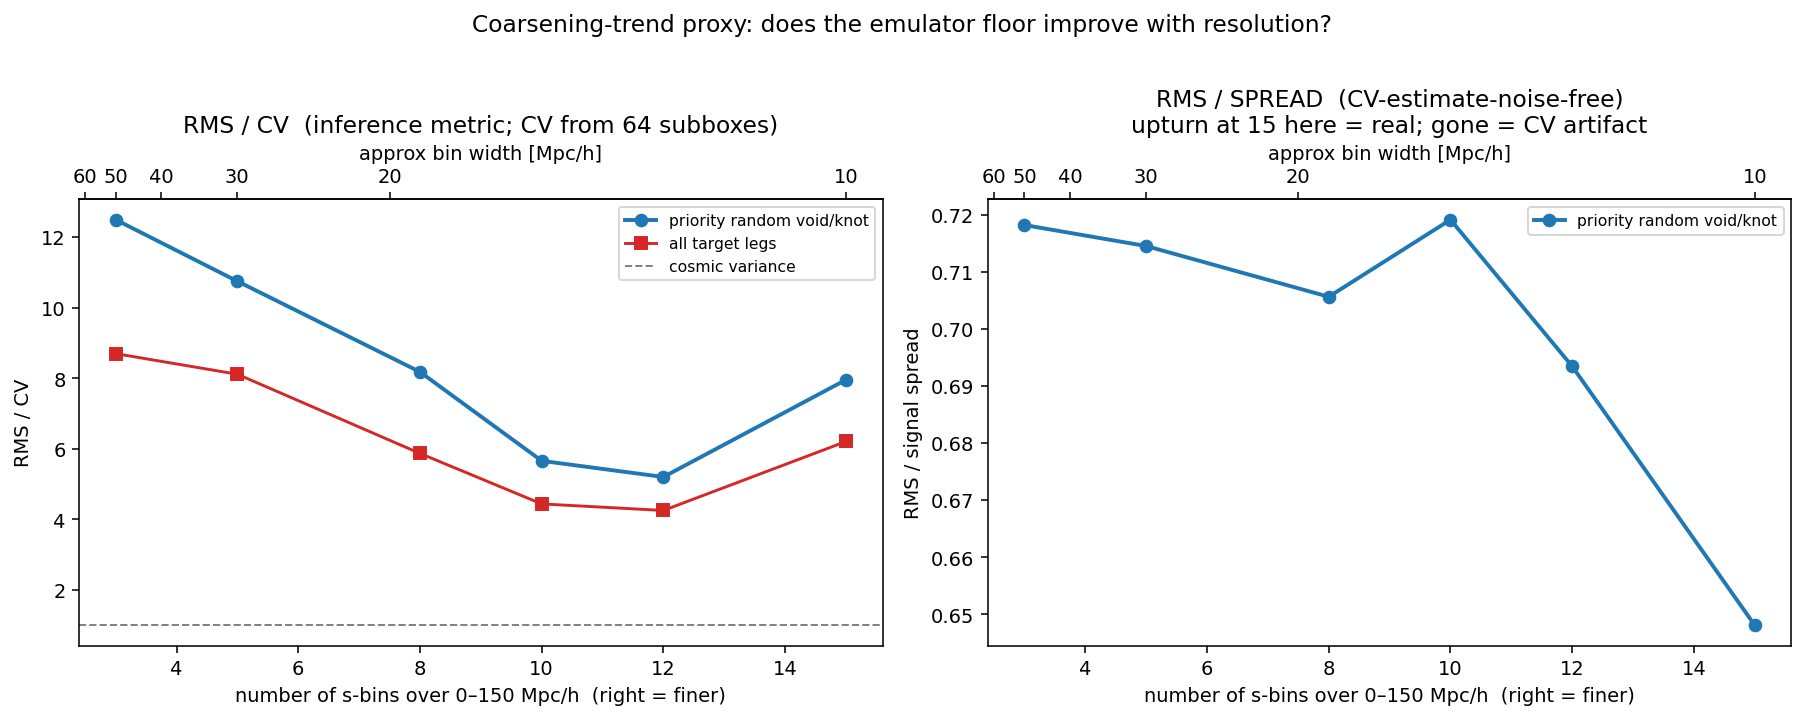
\includegraphics[width=0.85\textwidth]{binning_proxy.png}
\caption{Coarsening-trend proxy. RMS/CV (left) is U-shaped, but the upturn at the
finest bins vanishes in RMS/spread (right), which is flat --- so the upturn was a
CV-denominator artifact and finer binning is not a strong lever ($\lesssim$10\% over
$50\!\to\!10\Mpch$, far short of the order-of-magnitude needed).}
\label{fig:binproxy}
\end{figure}

\subsection{Resolution: the floor is monopole-vs-quadrupole}
Splitting the within-cosmology floor by leg (Fig.~\ref{fig:dvr}) reveals the real
structure: it is not data-vs-random but \textbf{monopole-vs-quadrupole}. The
\emph{monopoles} (both data and random) emulate well, several at or below cosmic
variance; the \emph{quadrupoles} carry the entire floor. This matches the
independent iteration experiment (random quadrupoles are noise-limited at 3
iterations, improving toward 10): \textbf{the quadrupole floor is the 3-iteration
ASTRA label noise on the velocity-dependent $\ell=2$ signal}, not binning, model, or
HOD count. The ``$\sim$6--8$\times$ floor'' quoted from aggregate metrics was great
monopoles averaged with noisy quadrupoles.

\begin{figure}[h]\centering
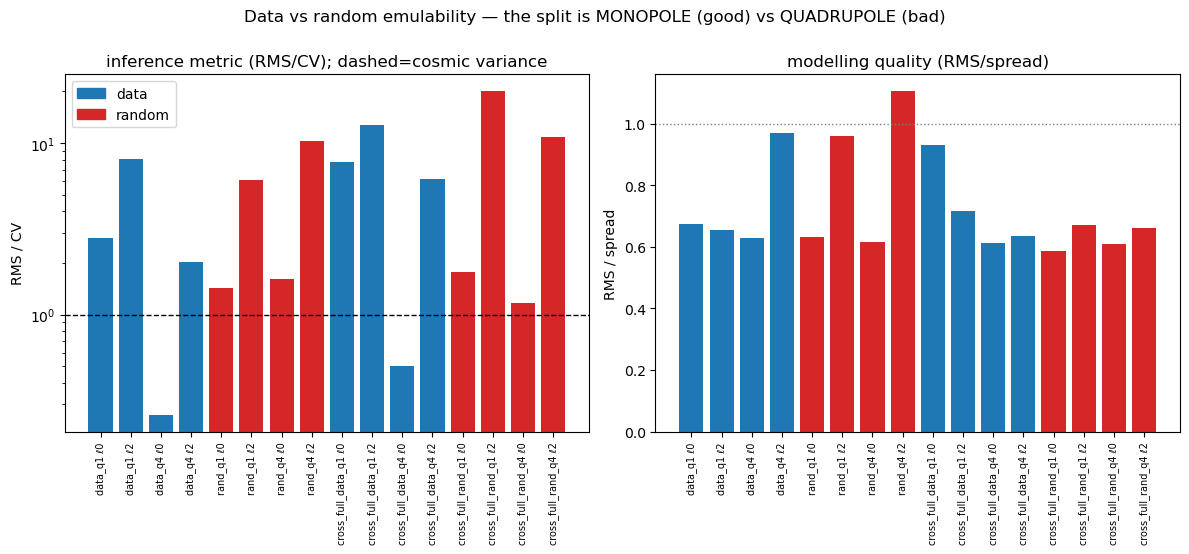
\includegraphics[width=0.95\textwidth]{data_vs_random.png}
\caption{Per-leg within-cosmology emulability. The split is monopole (good) vs
quadrupole (bad), in \emph{both} data and random families. Monopoles are the
inference-ready legs; the quadrupole floor is iteration-noise-limited.}
\label{fig:dvr}
\end{figure}

\subsection{A CV-denominator correction}
While building the inference test we found a bug in the cosmic-variance helpers:
they read the per-cosmology \emph{mean} multipole (\code{xi0}, 9 samples) instead of
the per-subbox array (\code{xi0\_all}, 576 pooled samples), so ``CV'' was a
cosmology-variation, not cosmic variance. After the fix every absolute $\times$CV
number shifts by $\sim$0.6--5$\times$ per bin, but \emph{all relative conclusions
above hold} (they compare ratios with the same denominator on both sides), as do the
RMS/spread results (which never use CV). The corrected absolute numbers are quoted in
the next section.

%======================================================================
\section{Results II: most-informative scales and cosmology response}
Two model-free diagnostics characterise where the cosmological information lives and
how the legs respond to cosmology, using all 19 cosmologies on disk.

\paragraph{Scale.} A cumulative-information analysis (Fig.~\ref{fig:scale}) shows the
\textbf{monopole} cosmological information is concentrated at \textbf{small scales}
($\sim$50\% by $s\!\approx\!30$--$55\Mpch$), while the \textbf{quadrupole}
information sits at \textbf{large scales} ($\gtrsim100\Mpch$, the Kaiser regime).
Small scales carry both the highest cosmology signal and the highest HOD nuisance ---
which is why the emulator is needed there.

\paragraph{Response.} Single-parameter Fisher $\pm$ pairs (Fig.~\ref{fig:resp}),
HOD-marginalised and split by environment, give the clean attribution the broad
Latin-hypercube cannot: $\omega_{\rm cdm}$ is the largest, cleanest mover;
$\sigma_8$/amplitude is bias-degenerate (at fixed number density a \emph{lower}
$\sigma_8$ can give a \emph{higher} $\xi$); and void and knot respond
\emph{differently} to each parameter --- the degeneracy-breaking that motivates
ASTRA, visible by eye.

\begin{figure}[h]\centering
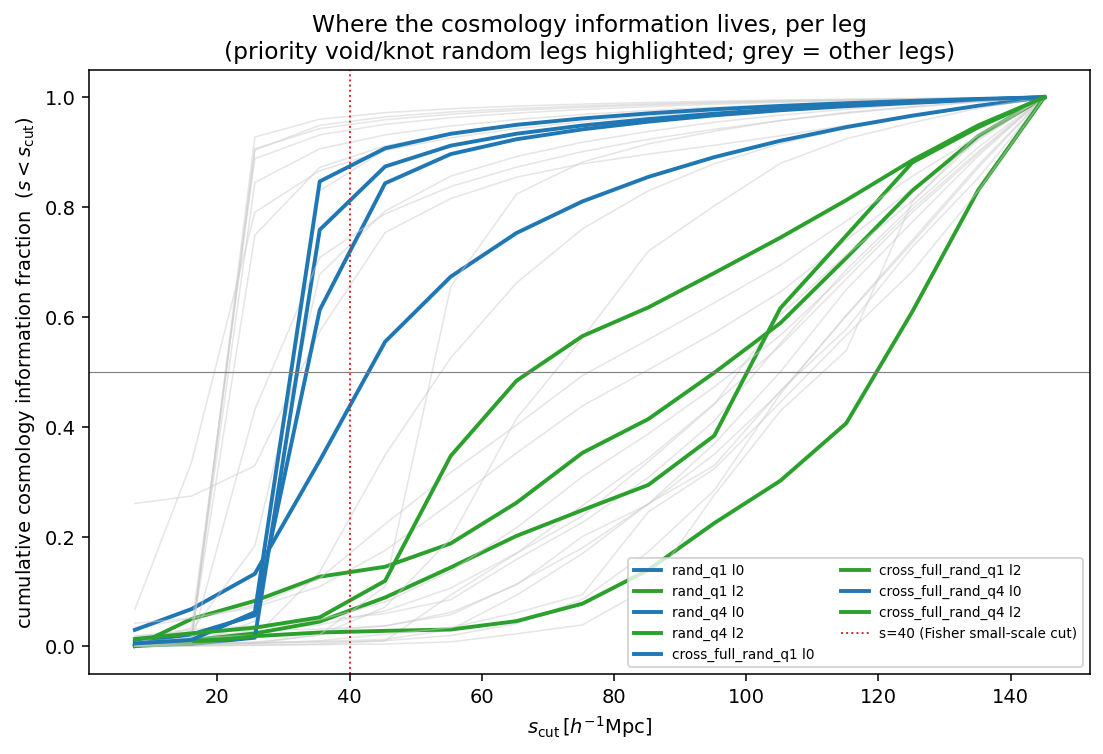
\includegraphics[width=0.6\textwidth]{scale_information_cumulative.png}
\caption{Cumulative cosmology-information fraction vs scale cut, per leg. Monopole
($\ell=0$) curves saturate by $s\!\sim\!50\Mpch$ (small-scale information);
quadrupole ($\ell=2$) curves rise slowly to large scales.}
\label{fig:scale}
\end{figure}

\begin{figure}[h]\centering
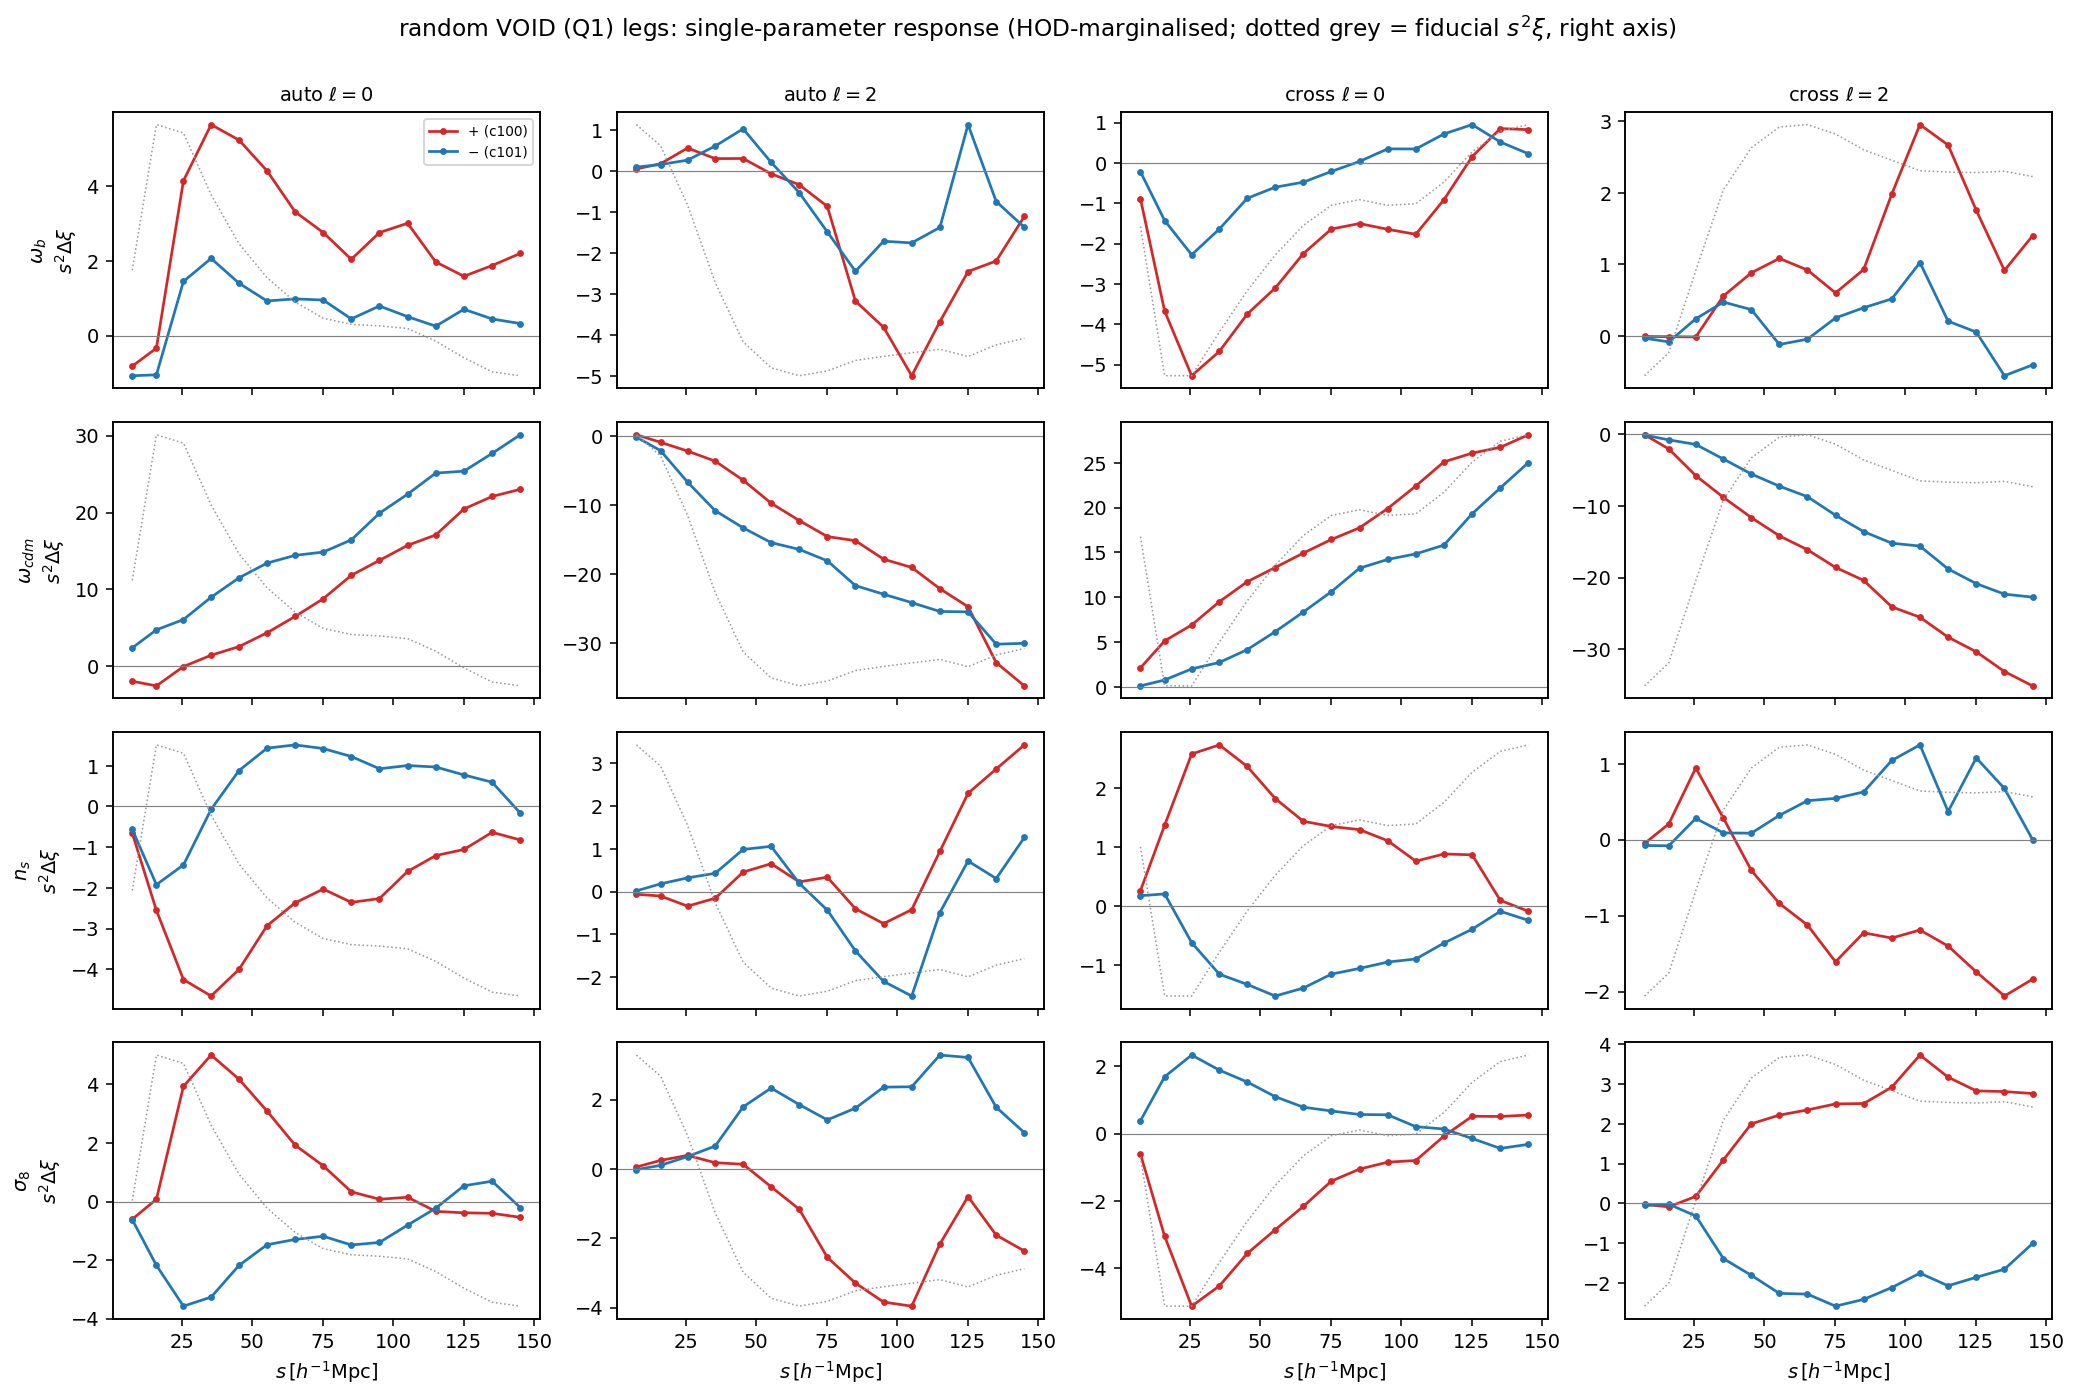
\includegraphics[width=0.49\textwidth]{param_response_rand_void.png}\hfill
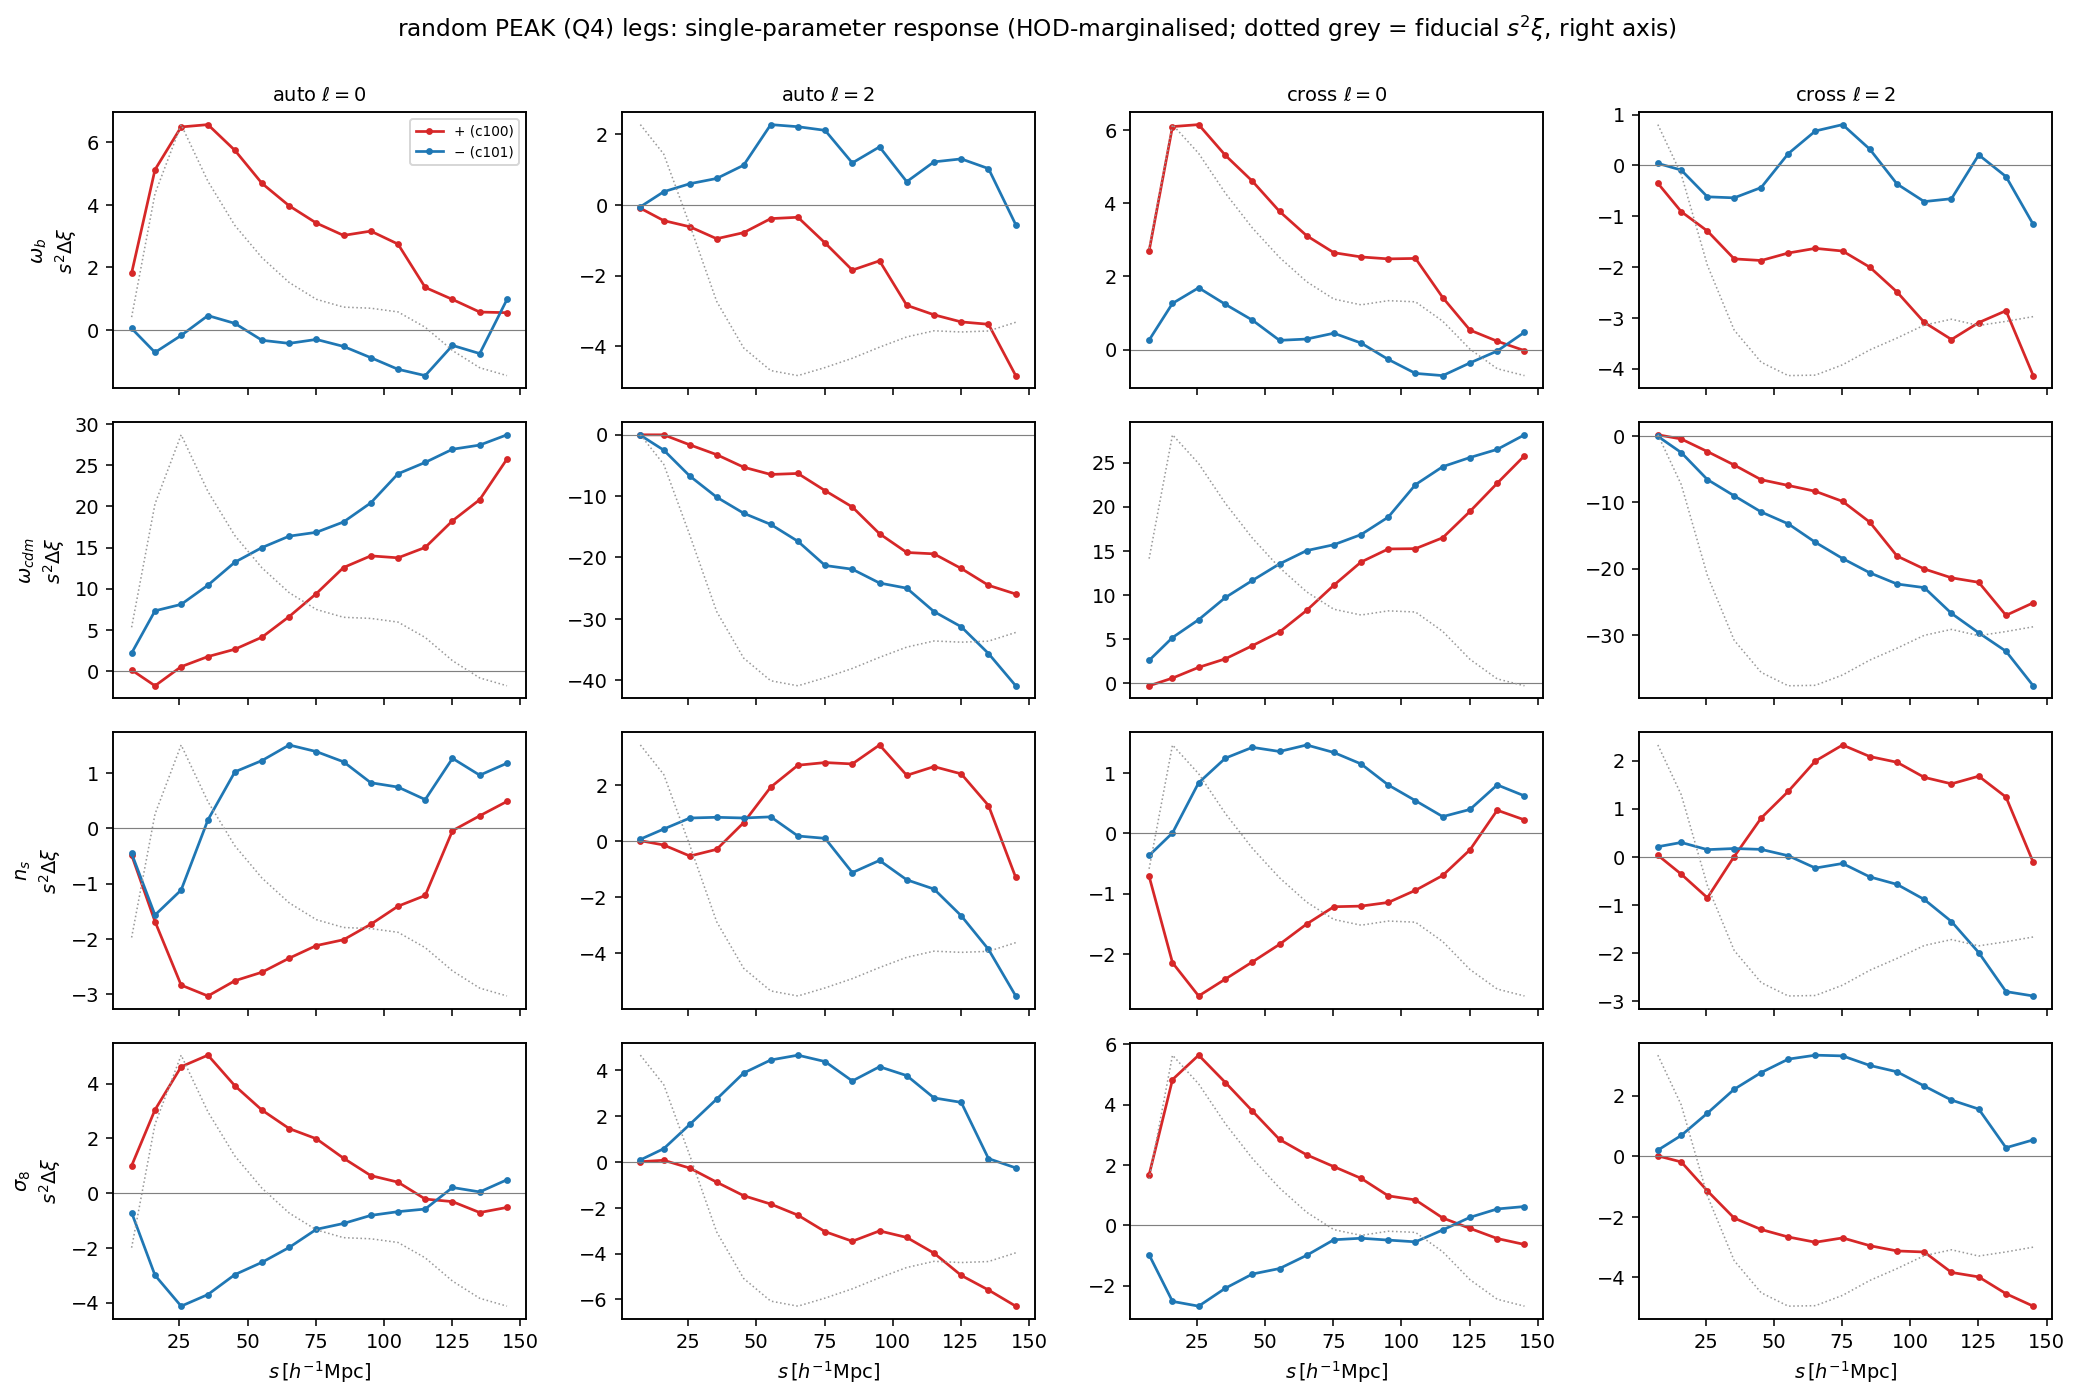
\includegraphics[width=0.49\textwidth]{param_response_rand_peak.png}
\caption{Single-parameter response of the random void (left) and knot (right) legs
from the Fisher $\pm$ pairs (shift $s^2\Delta\xi$ for $+$/$-$; rows are the four
LCDM parameters). The $+$/$-$ mirror symmetry indicates a clean linear response;
$\omega_{\rm cdm}$ dominates; void and knot differ.}
\label{fig:resp}
\end{figure}

%======================================================================
\section{Results III: monopole emulator and inference prototype}
Guided by the floor result, we built the inference-ready piece: a \textbf{monopole}
forward model and a SUNBIRD-style recovery test, both on the legs that are clean
(the void \emph{data} monopoles are excluded --- near their $\xi$ zero-crossing the
CV vanishes and RMS/CV diverges).

\paragraph{Cross-cosmology accuracy (the gate).} The corrected monopole
leave-one-cosmology-out (Fig.~\ref{fig:monoloco}) is a textbook interpolation-vs-
extrapolation split: the nine Fisher cosmologies (dense LCDM neighbourhood) sit at
\textbf{$\sim$1.1$\times$CV} (\code{c000} at 1.0$\times$, i.e.\ at cosmic variance),
while the ten broad tier-3 cosmologies are extrapolation-limited at
\textbf{$\sim$18$\times$CV}. So a monopole inference is genuinely inference-grade
\emph{near LCDM today}; the broad prior needs the campaign's coverage.

\paragraph{Inference recovery.} The likelihood uses the emulator $\mu(\theta)$, the
subbox $C_{\rm CV}$, and an emulator-error $C_{\rm emu}$ from the Fisher-set LOCO
residuals, with \code{emcee} over the four LCDM parameters (HOD fixed = prototype).
Two mocks (Fig.~\ref{fig:corner}):
\begin{itemize}
\item \textbf{Synthetic} ($\mu$ at a displaced cosmology $+$ a draw from
  $C_{\rm CV}\!+\!C_{\rm emu}$): $\chi^2/{\rm dof}=0.55$, all four parameters
  recovered within $1\sigma$ at the displaced truth --- the
  sampler/likelihood/emulator-gradient \textbf{machinery is validated}.
\item \textbf{Real \code{c000}} ($C_{\rm tot}=C_{\rm CV}+C_{\rm emu}+C_{\rm label}$):
  the calibration removes the gross bias of an earlier broken attempt
  ($n_s$ from $-30\sigma$ to $-1.7\sigma$), but $\chi^2/{\rm dof}=13.5$ and
  $\omega_b$ at $+3.2\sigma$ remain --- residual per-run emulator bias beyond the
  averaged $C_{\rm emu}$, plus the fundamental same-phase-mock limitation (no
  independent realisation is available under the no-new-HOD constraint).
\end{itemize}

\begin{figure}[h]\centering
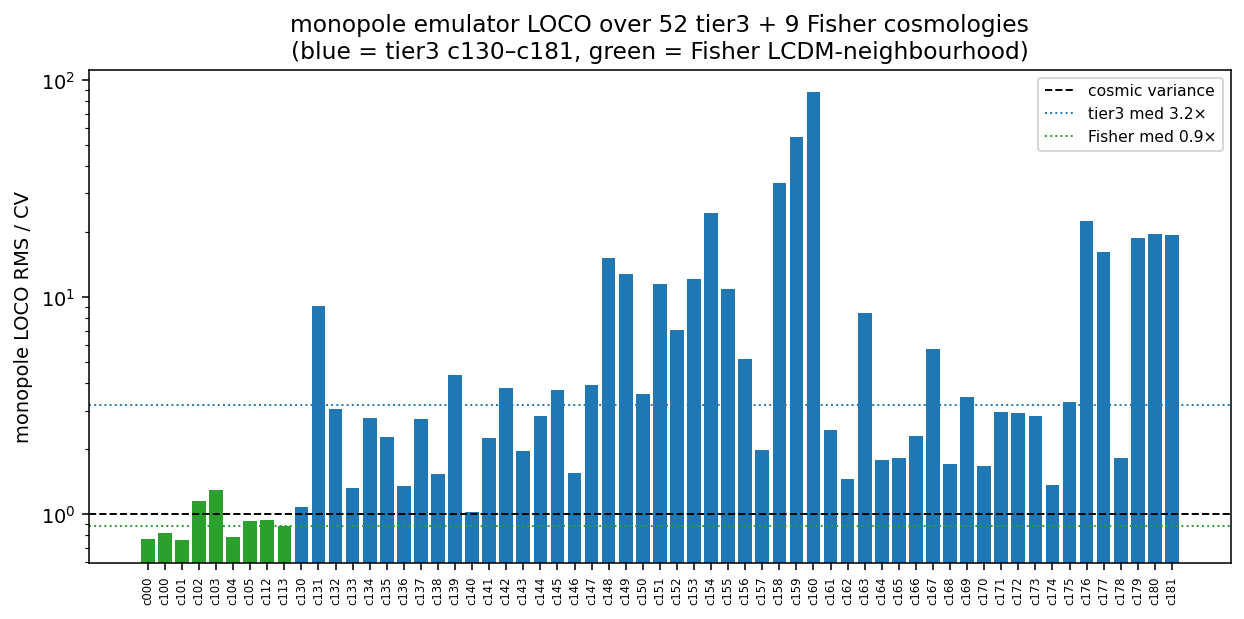
\includegraphics[width=0.66\textwidth]{monopole_loco.png}
\caption{Monopole emulator leave-one-cosmology-out floor (corrected CV). Green =
the nine Fisher LCDM-neighbourhood cosmologies ($\sim$1.1$\times$CV, interpolation);
blue = the ten broad tier-3 cosmologies ($\sim$18$\times$CV, extrapolation). The gap
is the cosmology-coverage gate.}
\label{fig:monoloco}
\end{figure}

\begin{figure}[h]\centering
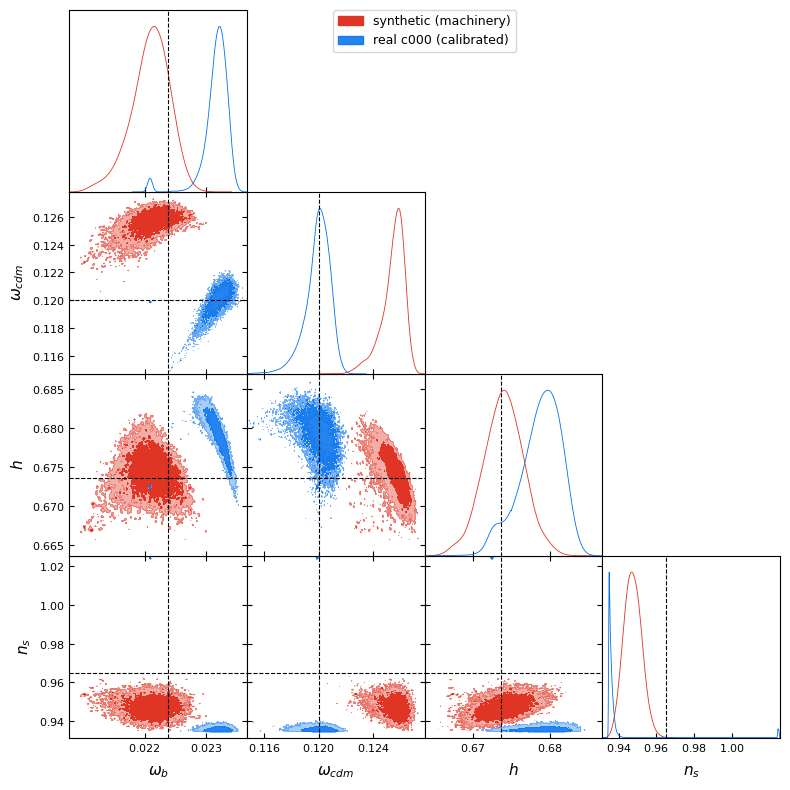
\includegraphics[width=0.66\textwidth]{inference_monopole_corner.png}
\caption{Recovery test (four LCDM parameters; dashed black $=$ \code{c000} truth).
Red: synthetic mock --- recovers the displaced injection within $1\sigma$
($\chi^2/{\rm dof}=0.55$), validating the pipeline. Blue: real \code{c000} mock with
calibrated covariance --- much improved but not yet clean
($\chi^2/{\rm dof}=13.5$), limited by per-run emulator realism.}
\label{fig:corner}
\end{figure}

%======================================================================
\section{The expanded cosmology grid and its new parameters}
A detail that drives everything below: the \emph{Fisher} grid (\code{c000} and
\code{c100}--\code{c113}, the LCDM neighbourhood) varies only the \textbf{four}
$\Lambda$CDM parameters $\{\omega_b,\omega_{\rm cdm},n_s,\sigma_8\}$ around Planck
(with $h$, $A_s$ retuned), whereas the \emph{emulator block} \code{c130}--\code{c181}
is the AbacusSummit emulator Latin hypercube, which opens up the broader
$w_0w_a$CDM$+$ space. The eight parameters that vary across that block --- and hence
the eight cosmology inputs of the emulator --- are:
\begin{center}\small
\begin{tabular}{llll}
\toprule
parameter & meaning & block range & in Fisher grid?\\
\midrule
$\omega_b$        & baryon density          & 0.0207--0.0243 & yes\\
$\omega_{\rm cdm}$& cold dark matter density& 0.103--0.140   & yes\\
$h$               & Hubble parameter        & 0.57--0.75     & (via retuning)\\
$n_s$             & scalar spectral index   & 0.90--1.03     & yes\\
$\alpha_s$        & running $dn_s/d\ln k$    & $-0.038$--$0.038$ & no (fixed 0)\\
$N_{\rm ur}$      & ultra-relativistic species ($\sim N_{\rm eff}$) & 1.2--2.9 & no (fixed 2.03)\\
$w_0$             & dark-energy EoS today   & $-1.27$--$-0.73$ & no (fixed $-1$)\\
$w_a$             & EoS evolution           & $-0.63$--$0.62$  & no (fixed 0)\\
\bottomrule
\end{tabular}
\end{center}
$A_s$ is fixed across the block and $\sigma_8$ is a \emph{derived} quantity (a
function of the eight inputs), so it is carried as a label, not an input. Three
consequences shape the results:
\begin{enumerate}
\item \textbf{The cosmology space is genuinely 8-D.} Even 52 cosmologies give only
  $52^{1/8}\!\approx\!1.7$ points per dimension --- dense in the interior, but the
  \emph{corners} of the hull stay sparse, so edge cosmologies extrapolate.
\item \textbf{Four of the eight ($\alpha_s,N_{\rm ur},w_0,w_a$) are new directions}
  the Fisher work never touched; the emulator is the only way to model them.
\item \textbf{Monopole-only data cannot constrain $w_0,w_a$ well.} The dark-energy
  EoS enters mainly through the expansion history / Alcock--Paczynski distortion,
  whose clean signature is anisotropic (the quadrupole); at fixed redshift the
  real-space monopole is largely degenerate in $w_0$--$w_a$. So a monopole inference
  pins $\omega_b,\omega_{\rm cdm},n_s$ but leaves $w_0,w_a$ loose until the
  quadrupole comes online.
\end{enumerate}

%======================================================================
\section{Results IV: the coverage run pays off}
The minimal coverage run --- \textbf{all 52 cosmologies $\times$ 20 maximin HODs
$\times$ 3 iterations} (the 10 pilot cosmologies reused; $\sim$840 new runs,
$\sim$490 node-hours), via \code{select\_tier3\_min.py} and
\code{queue/launch\_tier3\_minimal.sh} --- completed (it cleared in $\sim$12 h once
an overnight backfill window opened, far faster than the fairshare rate implied).
Re-running the monopole leave-one-cosmology-out over the now-filled grid
(Fig.~\ref{fig:monoloco52}) confirms the central hypothesis:
\begin{center}\small
\begin{tabular}{lcc}
\toprule
monopole LOCO (per-cosmology median RMS/CV) & 10 cosmologies & \textbf{52 cosmologies}\\
\midrule
tier-3 broad prior & $\sim$18$\times$ & \textbf{3.3$\times$}\\
Fisher LCDM neighbourhood & 1.1$\times$ & 0.9$\times$ (unchanged)\\
\bottomrule
\end{tabular}
\end{center}
Densening the hull $10\!\to\!52$ pulls the broad-prior emulator from extrapolation
($\sim$18$\times$) down by $\sim$5.5$\times$ toward the interpolation floor: now
\textbf{44\% of tier-3 cosmologies are below 3$\times$CV and 65\% below 5$\times$},
and the 10 original pilot cosmologies went from $\sim$18$\times$ to 3.8$\times$
(e.g.\ \code{c130} 1.1$\times$, \code{c140} 1.2$\times$). \textbf{Coverage was the
gate.} The residual outliers (\code{c160} 87$\times$, \code{c180} 24$\times$) are the
8-D hull \emph{corners} of \S\,8 --- where 52 points are still too sparse. (Note the
per-cosmology \emph{median}, 3.3$\times$, is the representative number; an RMS pooled
over all runs is dominated by those few outliers and reads higher.)

\begin{figure}[h]\centering
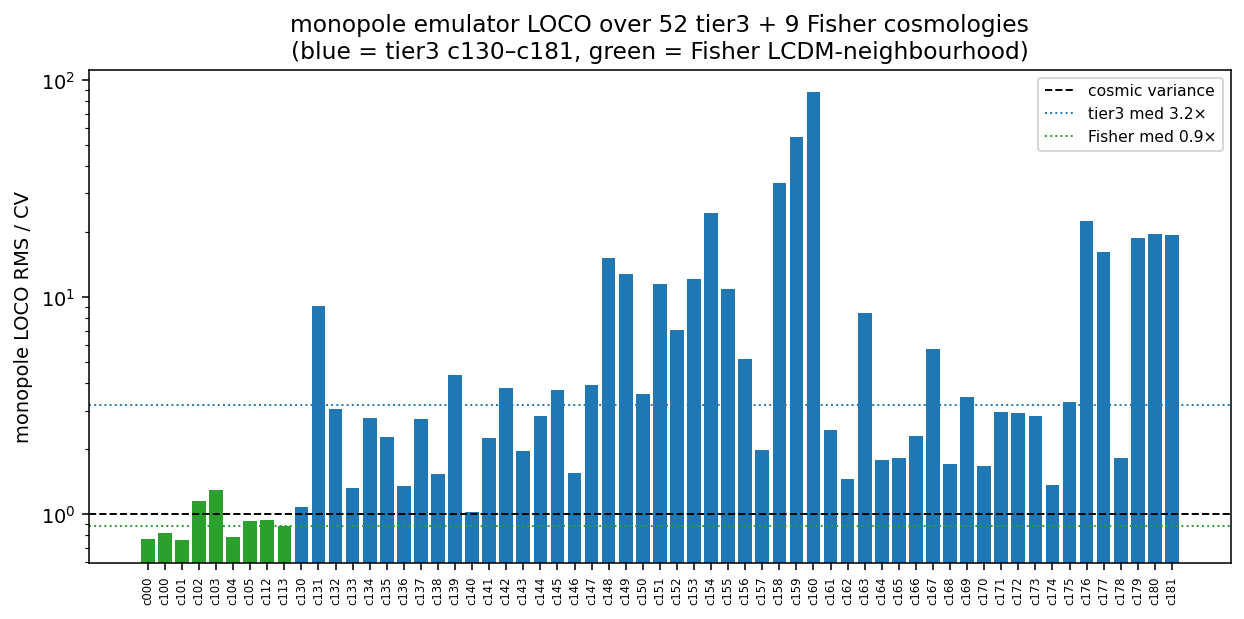
\includegraphics[width=0.78\textwidth]{monopole_loco.png}
\caption{Monopole emulator LOCO over the filled grid (52 tier-3 + 9 Fisher
cosmologies, corrected CV). Green = Fisher LCDM neighbourhood ($\sim$0.9$\times$CV,
interpolation); blue = tier-3 broad prior (median 3.3$\times$, was $\sim$18$\times$
at 10 cosmologies). A few 8-D hull corners (e.g.\ \code{c160}) remain
extrapolation-limited.}
\label{fig:monoloco52}
\end{figure}

\paragraph{Broad-prior inference (prototype).} With the broad directions now
modelled, \code{inference\_monopole.py} was generalised (\code{--mock-cosmo},
\code{--fit lcdm|broad}) and a tier-3 cosmology (\code{c130}) recovered over the six
monopole-relevant parameters $\{\omega_b,\omega_{\rm cdm},h,n_s,w_0,w_a\}$
(Fig.~\ref{fig:c130corner}). This was simply \emph{impossible} before the coverage
run --- the broad directions had no gradient support. Results:
\begin{itemize}
\item \textbf{Synthetic mock} (inject a displaced point, recover): $\chi^2/{\rm
  dof}=0.34$ and \emph{all six} parameters --- \emph{including} $w_0,w_a$ ---
  recovered within $\sim1\sigma$. The broad-prior sampler/likelihood/emulator-gradient
  machinery is validated over the full $w_0w_a$CDM$+$ subspace.
\item \textbf{Real \code{c130} mock}: $\chi^2/{\rm dof}=1.72$ --- far better-calibrated
  than the LCDM-only $c000$ test ($13.5$), because the honest (large) tier-3
  $C_{\rm emu}$ gives a realistic error budget. $\omega_{\rm cdm}$ and $h$ recover
  well ($+0.1\sigma$, $-0.4\sigma$); $\omega_b,n_s,w_0$ are biased at $\sim$3$\sigma$
  (residual per-run emulator bias); and $w_a$ is loose ($\pm0.22$), exactly as
  expected --- the monopole alone cannot pin the dark-energy EoS.
\end{itemize}
Two caveats remain: for a tier-3 mock $C_{\rm emu}/C_{\rm CV}\!\sim\!16$ (inflated by
the hull-corner outliers), so broad-prior inference is currently emulator-error-,
not cosmic-variance-limited; and the same-phase-mock limitation persists. A
neighbourhood-matched $C_{\rm emu}$ and the quadrupole are what tighten the test and
sharpen $w_0,w_a$.

\begin{figure}[h]\centering
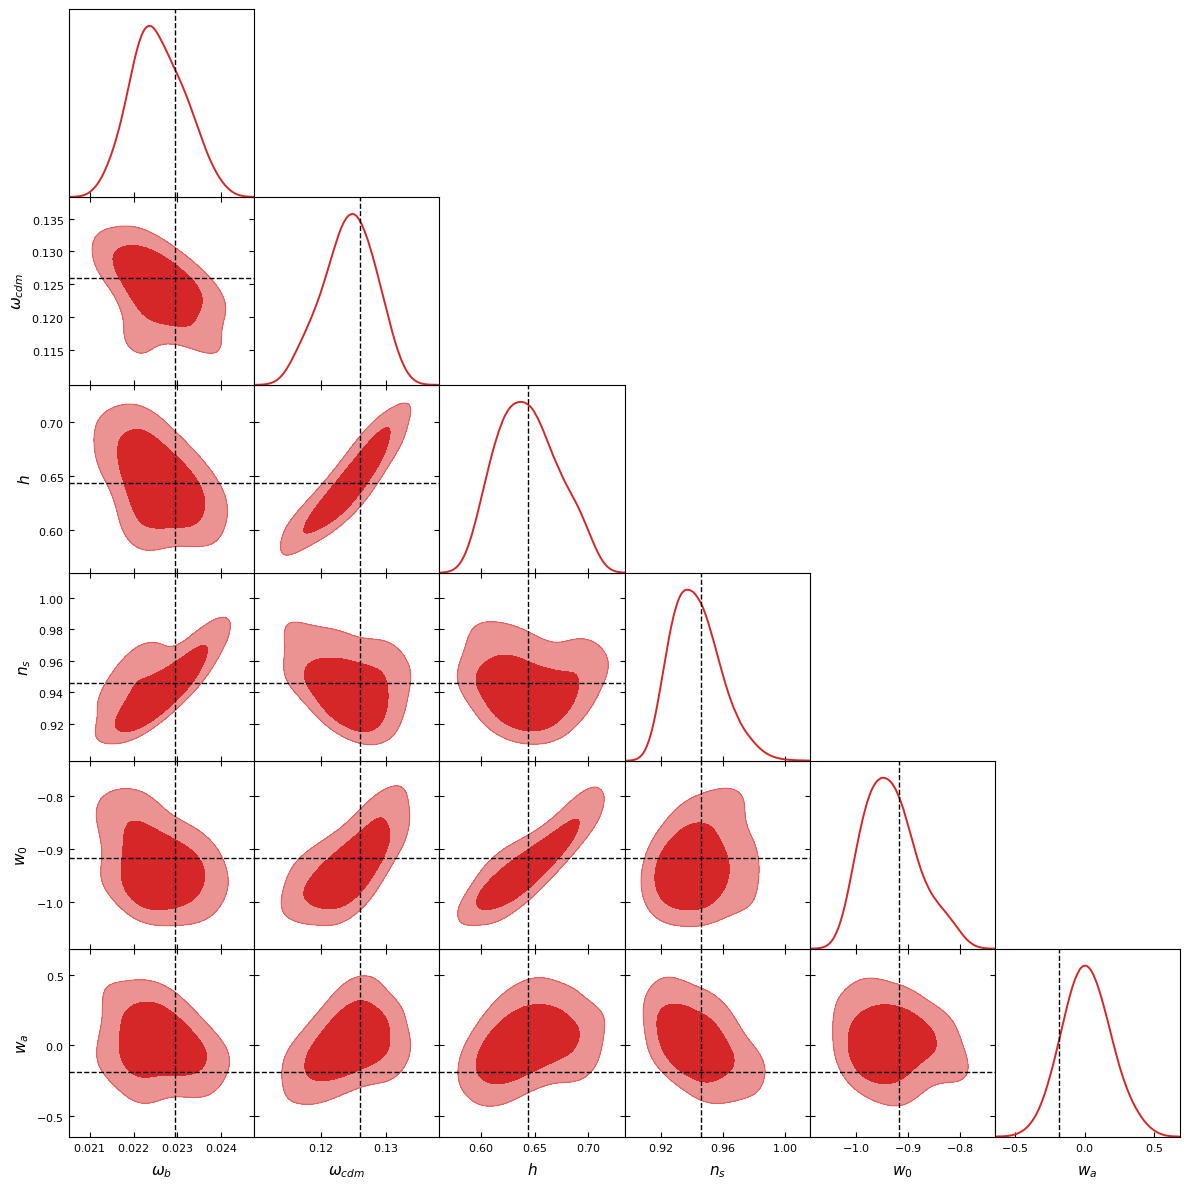
\includegraphics[width=0.49\textwidth]{inference_c130_broad_synth.png}\hfill
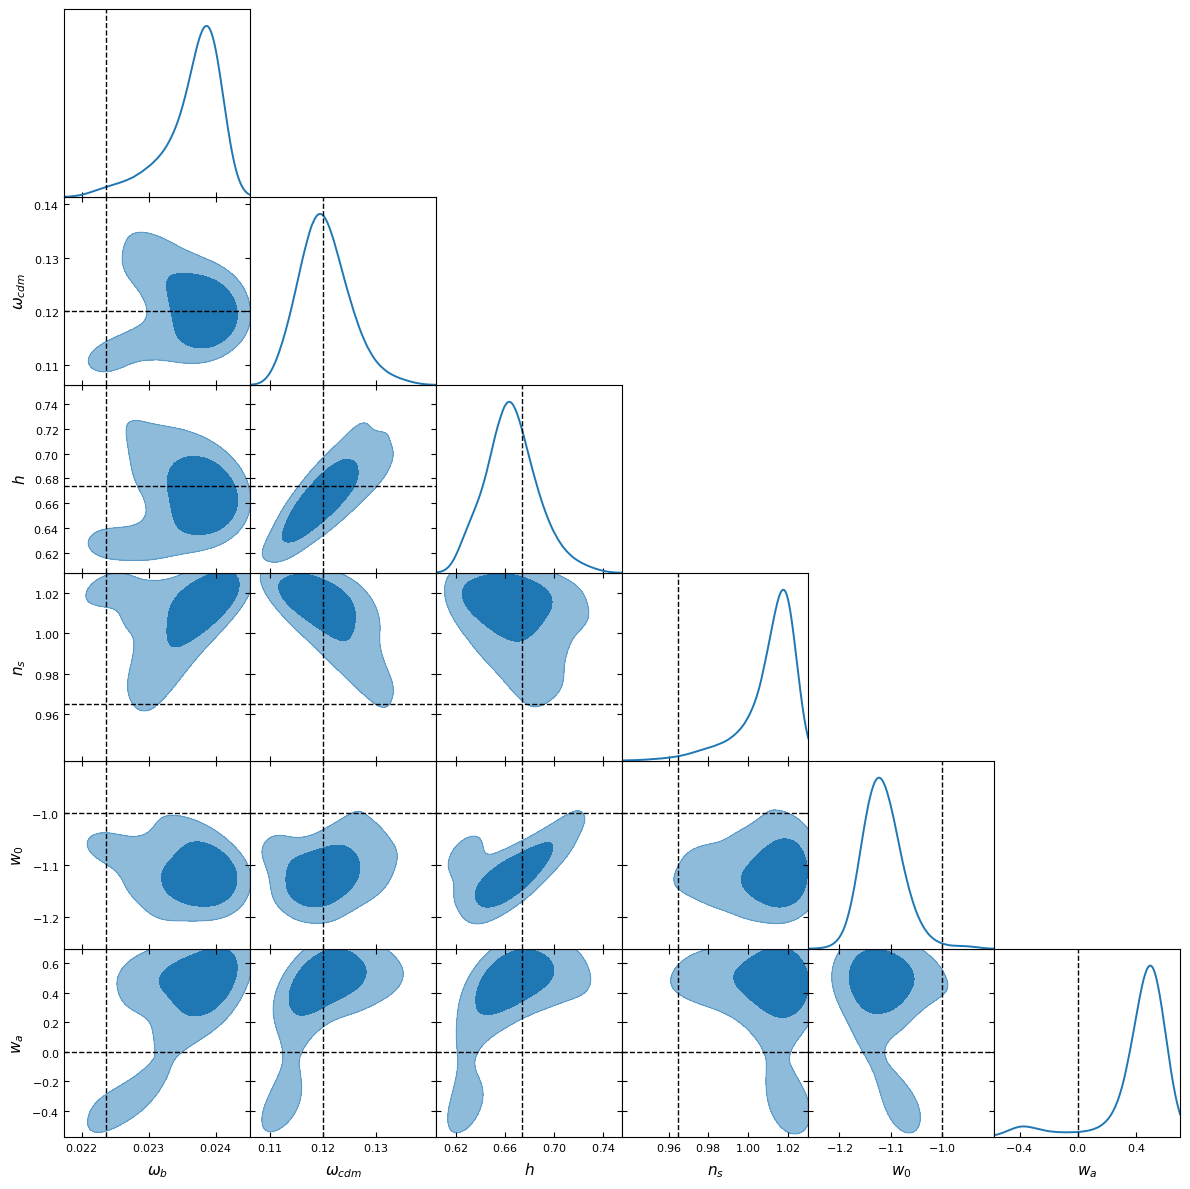
\includegraphics[width=0.49\textwidth]{inference_c130_broad_real.png}
\caption{Broad-prior recovery of \code{c130} over six parameters (68\%/95\% filled
contours; dashed black $=$ truth). \emph{Left, synthetic mock} (red): recovers within
$\sim1\sigma$ of its (displaced) injected truth at $\chi^2/{\rm dof}=0.34$ ---
validates the machinery over the $w_0w_a$CDM$+$ subspace. \emph{Right, real \code{c130}}
(blue, $\chi^2/{\rm dof}=1.72$): $\omega_{\rm cdm},h$ recovered; $\omega_b,n_s,w_0$
biased $\sim$3$\sigma$ (residual per-run emulator bias); $w_a$ loose --- monopole-only
cannot constrain the dark-energy EoS.}
\label{fig:c130corner}
\end{figure}

%======================================================================
\section{Results V: the ASTRA value-add is emulator-gated --- and CV-weighting
partly unlocks it}
The project's central claim is that splitting by environment adds cosmological
information beyond the plain two-point function. We test it directly
(\code{inference\_astra\_valueadd.py}): an identical synthetic recovery for two data
vectors --- \textbf{baseline} (\code{tpcf\_full\_data}, the standard 2PCF) vs
\textbf{full $+$ six ASTRA quantile monopoles} --- same mock, emulator and covariance
$C=C_{\rm CV}+C_{\rm emu}$, so only the vector differs.

\paragraph{First attempt (noise-weighted emulator): null.} The quantiles added
nothing ($\sigma$ ratios 1.00/1.04/1.04/0.95). \emph{Not} for lack of information:
the quantile-leg emulator error was $C_{\rm emu}/C_{\rm CV}\!\approx\!4.6$ (median),
$\sim$22$\times$ in variance, so $C_{\rm CV}+C_{\rm emu}$ down-weighted the quantiles
$\sim$22$\times$ and buried their (real) signal. This reconciles with the Fisher work:
with a \emph{perfect} emulator ($C=C_{\rm CV}$) the documented value-add is
1.3--2.4$\times$/param; in \emph{real} inference it evaporated because the environment
legs were not emulated to $\ll$ CV.

\paragraph{The fix --- CV-weighted loss.} An architecture/loss sweep
(\code{emulator\_arch\_sweep.py}, Fig.~\ref{fig:archsweep}) found the culprit: the
emulator was trained with an \emph{iteration-noise}-weighted loss ($1/\sigma_{\rm
iter}^2$), which \emph{down-weights} the (per-iteration-noisy) quantile legs, so the
joint MLP neglected them (cross-cosmology RMS/CV $\sim$31 on the quantile legs).
Switching to a \textbf{CV-weighted loss} ($1/C_{\rm CV}$, the inference metric) cuts
that to $\sim$2$\times$CV --- a \textbf{$\sim$15$\times$ improvement}, and every leg
improves (it is the correct metric, not a trade-off). Per-leg networks add nothing
beyond the weighting. We adopted CV-weighting in \code{train\_emulator}.

\paragraph{Re-test (CV-weighted): partially unlocked.} $C_{\rm emu}/C_{\rm CV}$ drops
$4.6\!\to\!2.65$, \emph{all} constraints tighten (the baseline 2PCF alone improves
$\sim$1.5$\times$ on $\omega_{\rm cdm},h$ from the better emulator), and the ASTRA
value-add \emph{emerges from null} (Fig.~\ref{fig:valueadd}):
\begin{center}\small
\begin{tabular}{lccc}
\toprule
 & baseline 2PCF & full $+$ ASTRA & tighter by\\
\midrule
$\sigma(\omega_b)$        & 0.00102 & 0.00110 & 0.93$\times$\\
$\sigma(\omega_{\rm cdm})$& 0.00664 & 0.00570 & \textbf{1.16$\times$}\\
$\sigma(h)$               & 0.0123  & 0.0112  & \textbf{1.10$\times$}\\
$\sigma(n_s)$             & 0.0354  & 0.0353  & 1.00$\times$\\
\bottomrule
\end{tabular}
\end{center}
Still short of the Fisher 1.3--2.4$\times$ because $C_{\rm emu}$ (2.65$\times$CV)
remains \emph{above} cosmic variance. But the \textbf{mechanism is now demonstrated:
the value-add grows as $C_{\rm emu}$ falls} (null at 4.6$\times$ $\to$ 1.16$\times$ at
2.65$\times$). Extrapolating, driving $C_{\rm emu}\!\ll\!$CV (the full campaign: more
iterations to kill the random/quadrupole label noise $+$ denser coverage) should
deliver the full gain. The campaign justification is now precise: \emph{each factor
$C_{\rm emu}$ drops below CV converts into ASTRA value-add}.

\begin{figure}[h]\centering
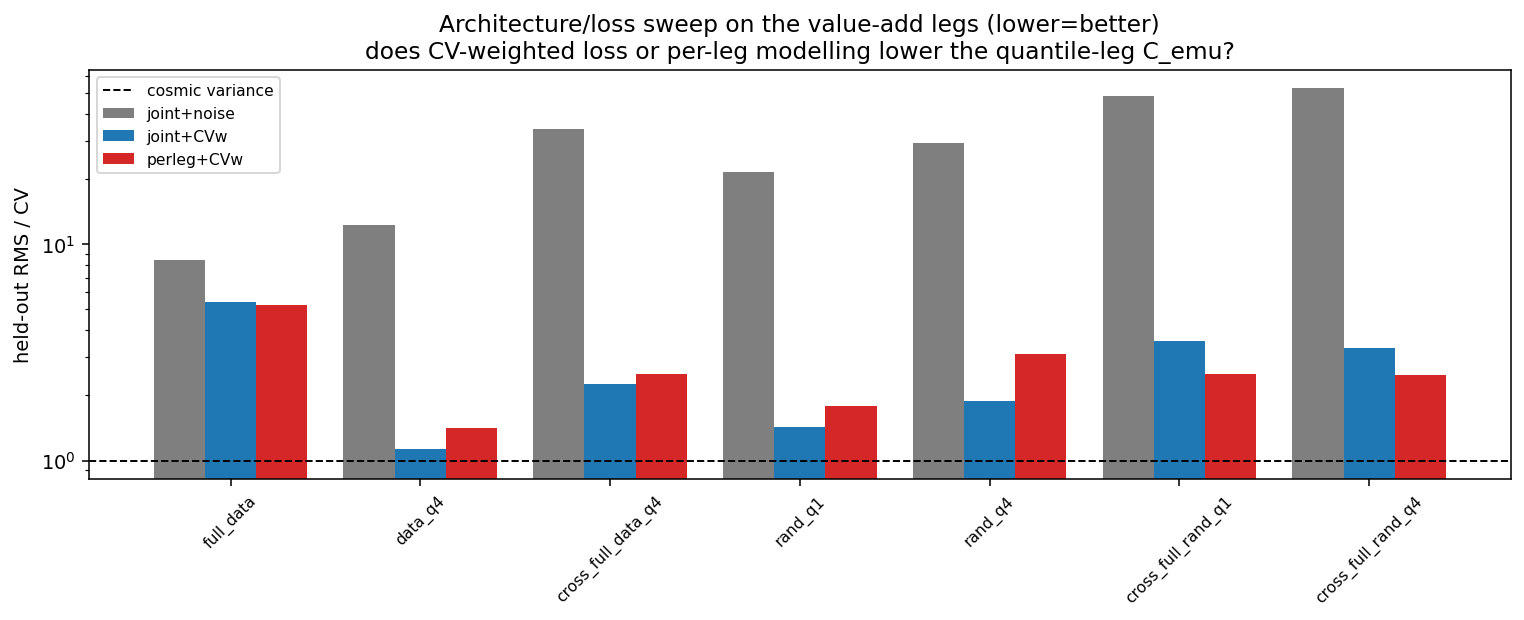
\includegraphics[width=0.92\textwidth]{arch_sweep.png}
\caption{Architecture/loss sweep on the value-add legs (cross-cosmology held-out
RMS/CV; lower=better). The iteration-noise-weighted loss (grey) starves the quantile
legs ($\sim$31$\times$CV median); a \textbf{CV-weighted loss} (blue) cuts them to
$\sim$2$\times$CV ($\sim$15$\times$ better), and per-leg networks (red) add nothing
beyond that. The loss weighting, not the architecture, was the lever.}
\label{fig:archsweep}
\end{figure}

\begin{figure}[h]\centering
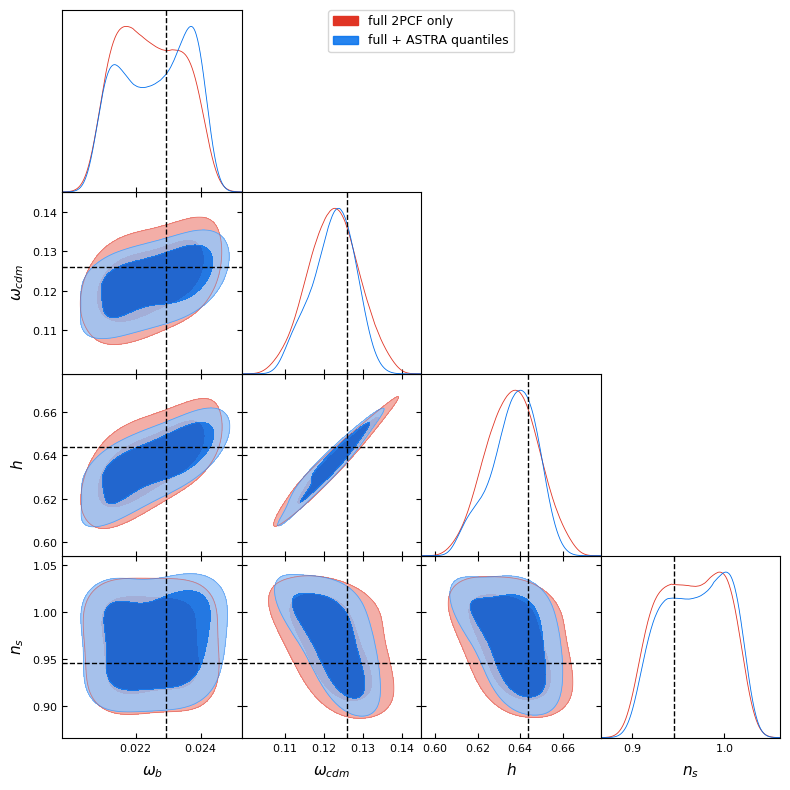
\includegraphics[width=0.62\textwidth]{astra_valueadd_corner.png}
\caption{ASTRA value-add with the CV-weighted emulator: full 2PCF (red) vs full $+$
ASTRA quantiles (blue), same mock/emulator/covariance (dashed $=$ truth). The blue
contours now sit \emph{inside} red for $\omega_{\rm cdm}$ and $h$ ($\sim$1.1$\times$),
where with the noise-weighted emulator they overlapped exactly. The full Fisher gain
awaits $C_{\rm emu}\!\ll\!$CV.}
\label{fig:valueadd}
\end{figure}

%======================================================================
\section{Results VI: HOD marginalisation and the real-vs-synthetic bias}
\paragraph{HOD marginalisation (\code{inference\_hodmarg.py}).} The prototype fixes
the 12 HOD parameters at truth --- optimistic. Re-running the c000 recovery with the
HOD \emph{marginalised} (vary cosmology $+$ all 12 HOD, project to the cosmology block)
inflates the cosmology errors only mildly: $\sigma(h)\times1.8$, $\sigma(n_s)\times1.6$,
$\sigma(\omega_b),\sigma(\omega_{\rm cdm})\times1.0$. The monopole environment legs
self-calibrate the HOD well enough that $\omega_b,\omega_{\rm cdm}$ are essentially
HOD-robust; $h,n_s$ (broadband-shape-degenerate with the HOD) take the modest hit.
This is far gentler than the 2--10$\times$ the joint-Fisher study warned of.

\paragraph{Why real-mock recoveries are biased while synthetic ones are not.} A clean,
recurring pattern: recoveries of a \emph{synthetic} mock (emulator at $\theta$ $+$ a
draw from $C$) are \emph{unbiased} ($\chi^2/{\rm dof}\!\sim\!0.3$--0.6, all params
$<1\sigma$), whereas recoveries of a \emph{real measured} mock (an actual c000/c130
run) are biased $\sim$2--3$\sigma$ and their HOD-fixed/marginalised contours are both
offset from truth. This is not the sampler: it is \textbf{per-run emulator realism}.
The emulator gives the smooth $(\theta_{\rm cosmo},\theta_{\rm HOD})\!\to\!\xi$ map; a
single measured realisation deviates from it (residual emulator bias $+$ 3-iteration
label noise $+$ the same-phase-mock limitation: ph000 only, so no independent
realisation to average against under the no-new-HOD constraint). The MCMC absorbs that
mismatch by shifting the cosmology. So the synthetic tests validate the machinery; the
real-mock bias is the same emulator-accuracy ($C_{\rm emu}$) limit, and shrinks as the
emulator improves. Independent-phase mocks would remove it entirely.

%======================================================================
\section{Results VII: emulator-aware greedy leg selection}
The old Fisher greedy ranked legs with $C=C_{\rm CV}$ (a perfect emulator) and crowned
the environment crosses. We redo it (\code{emulator\_greedy.py}) with the \emph{realistic}
budget $C(\alpha)=C_{\rm CV}+\alpha\,C_{\rm emu}$ (emulator-derived derivatives;
FoM$=\det(D_{\rm cosmo}^{\!\top}C^{-1}D_{\rm cosmo})^{1/2}$ over
$\{\omega_b,\omega_{\rm cdm},h,n_s\}$), greedily forward-selecting among 18 candidate
leg-blocks (full 2PCF $+$ the eight environment stems, $\ell=0$ and $\ell=2$), and sweep
$\alpha$ from 1 (current emulator, $C_{\rm emu}/C_{\rm CV}\!\approx\!7.6$) to 0 (perfect).

\paragraph{ASTRA's best leg beats the plain 2PCF --- even now.} At the current emulator
accuracy ($\alpha=1$) the single most informative leg is the \textbf{void $\times$
full-sample cross monopole} (\code{cross\_full\_rand\_q1}~$\ell0$), ahead of the plain
2PCF; the top $\sim$4 legs are stable across all $\alpha$ (void-cross $\ell0$, full
2PCF $\ell0{+}\ell2$, void-data $\ell0$). So a \emph{curated} ASTRA vector is the
strong choice today --- and refines the earlier value-add null, which diluted the gain
by adding all six legs indiscriminately (the noisy quadrupoles and q4-data legs do not
help at current accuracy).

\begin{center}\small
\begin{tabular}{lcc}
\toprule
leg (greedy rank) & $\alpha=1$ (now) & $\alpha=0$ (perfect)\\
\midrule
void$\times$full cross $\ell0$ & 1 & 2\\
full 2PCF $\ell0$              & 2 & 1\\
full 2PCF $\ell2$              & 3 & 3\\
void-data $\ell0$             & 4 & 5\\
void$\times$full-data cross $\ell0$ & 9 & \textbf{4}\ (switches on)\\
knot$\times$full-rand cross $\ell0$ & 13 & \textbf{9}\ (switches on)\\
knot-data $\ell2$            & 6 & 14\ (noise-favoured now)\\
\bottomrule
\end{tabular}
\end{center}

\paragraph{The campaign payoff is in the tail --- and the bar is high.} The
cumulative-FoM curves (Fig.~\ref{fig:greedy}) show a \emph{perfect} emulator reaching
$\sim$500$\times$ the first-leg FoM at the full vector versus $\sim$90$\times$ now ---
a \textbf{$\sim$5$\times$ FoM gap}, concentrated in the \emph{tail} legs (the extra
environment crosses and quadrupoles that climb in rank as $\alpha\to0$). Crucially the
$\alpha=1,0.3,0.1$ curves nearly overlap: reducing $C_{\rm emu}$ by $10\times$ barely
helps, and only $C_{\rm emu}\!\to\!0$ unlocks the $5\times$. Since
$C_{\rm emu}/C_{\rm CV}\!\approx\!7.6$ here, the campaign must drive the environment-leg
$C_{\rm emu}$ \textbf{well below cosmic variance ($\sim$0.1$\times$CV), not merely to
$\sim$CV} --- a sharper, more honest target than \S\,13 alone implied.

\begin{figure}[h]\centering
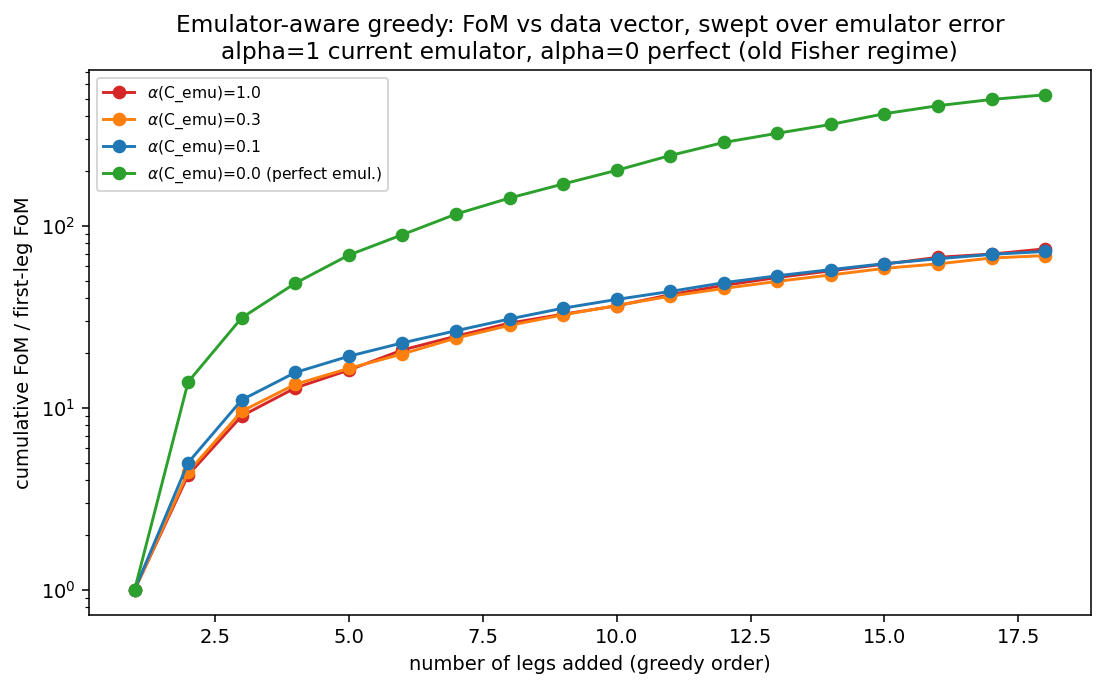
\includegraphics[width=0.66\textwidth]{emulator_greedy.png}
\caption{Emulator-aware greedy: cumulative FoM vs.\ data vector, swept over the
emulator-error scaling $\alpha$. A perfect emulator ($\alpha=0$, green) extracts
$\sim$5$\times$ more total FoM from the full ASTRA vector than the current one
($\alpha=1$, red); the $\alpha=1/0.3/0.1$ overlap shows the gain needs
$C_{\rm emu}\!\ll\!$CV. The tail legs (environment crosses, quadrupoles) are where the
campaign pays off.}
\label{fig:greedy}
\end{figure}

%======================================================================
\section{Results VIII: the curated vector realises the ASTRA value-add now}
Following the greedy, we built the curated vector \textbf{full 2PCF monopole $+$
void-random-cross monopole} (\code{inference\_curated.py}) and re-ran all three
inference tests. This is the strongest result of the note:
\begin{itemize}
\item \textbf{Value-add is now real:} adding the single best environment leg tightens
  $\sigma$ by $\omega_b\!\times\!1.19$, $\omega_{\rm cdm}\!\times\!1.63$,
  $h\!\times\!1.40$, $n_s\!\times\!1.72$ (Fig.~\ref{fig:curval}) --- versus $\times$1.1
  for the indiscriminate six-leg add. \emph{Curate to the best few legs; do not dump
  all of them.}
\item \textbf{Real c000 recovery is unbiased} (all params $<0.5\sigma$) --- the
  earlier $\sim$3$\sigma$ real-mock bias is gone, because both legs are well emulated.
\item \textbf{HOD-marginalisation is essentially free} ($\times$0.9--1.1).
\item \textbf{Why:} the leg diagnostic (\code{emulator\_leg\_diagnostic.py},
  Fig.~\ref{fig:legdiag}) shows the void-random-cross monopole emulates at
  \textbf{1.0$\times$CV in the LCDM neighbourhood} and 3.1$\times$ over the broad tier-3
  prior --- inference-grade where it matters, with the failures confined to the 8-D
  hull corners (e.g.\ \code{c160}).
\end{itemize}

\begin{figure}[h]\centering
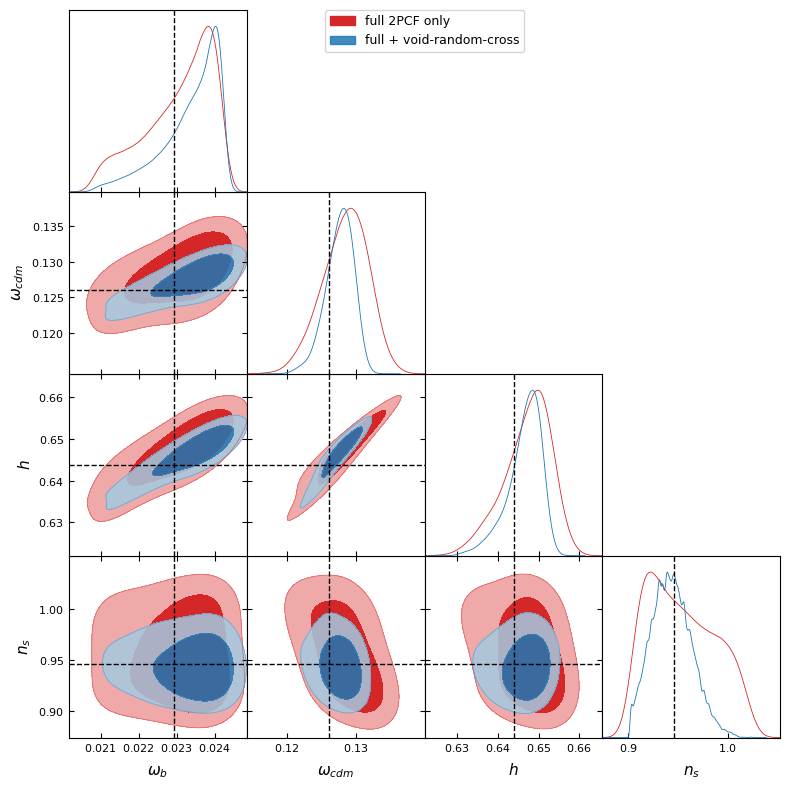
\includegraphics[width=0.49\textwidth]{inference_curated_valueadd.png}\hfill
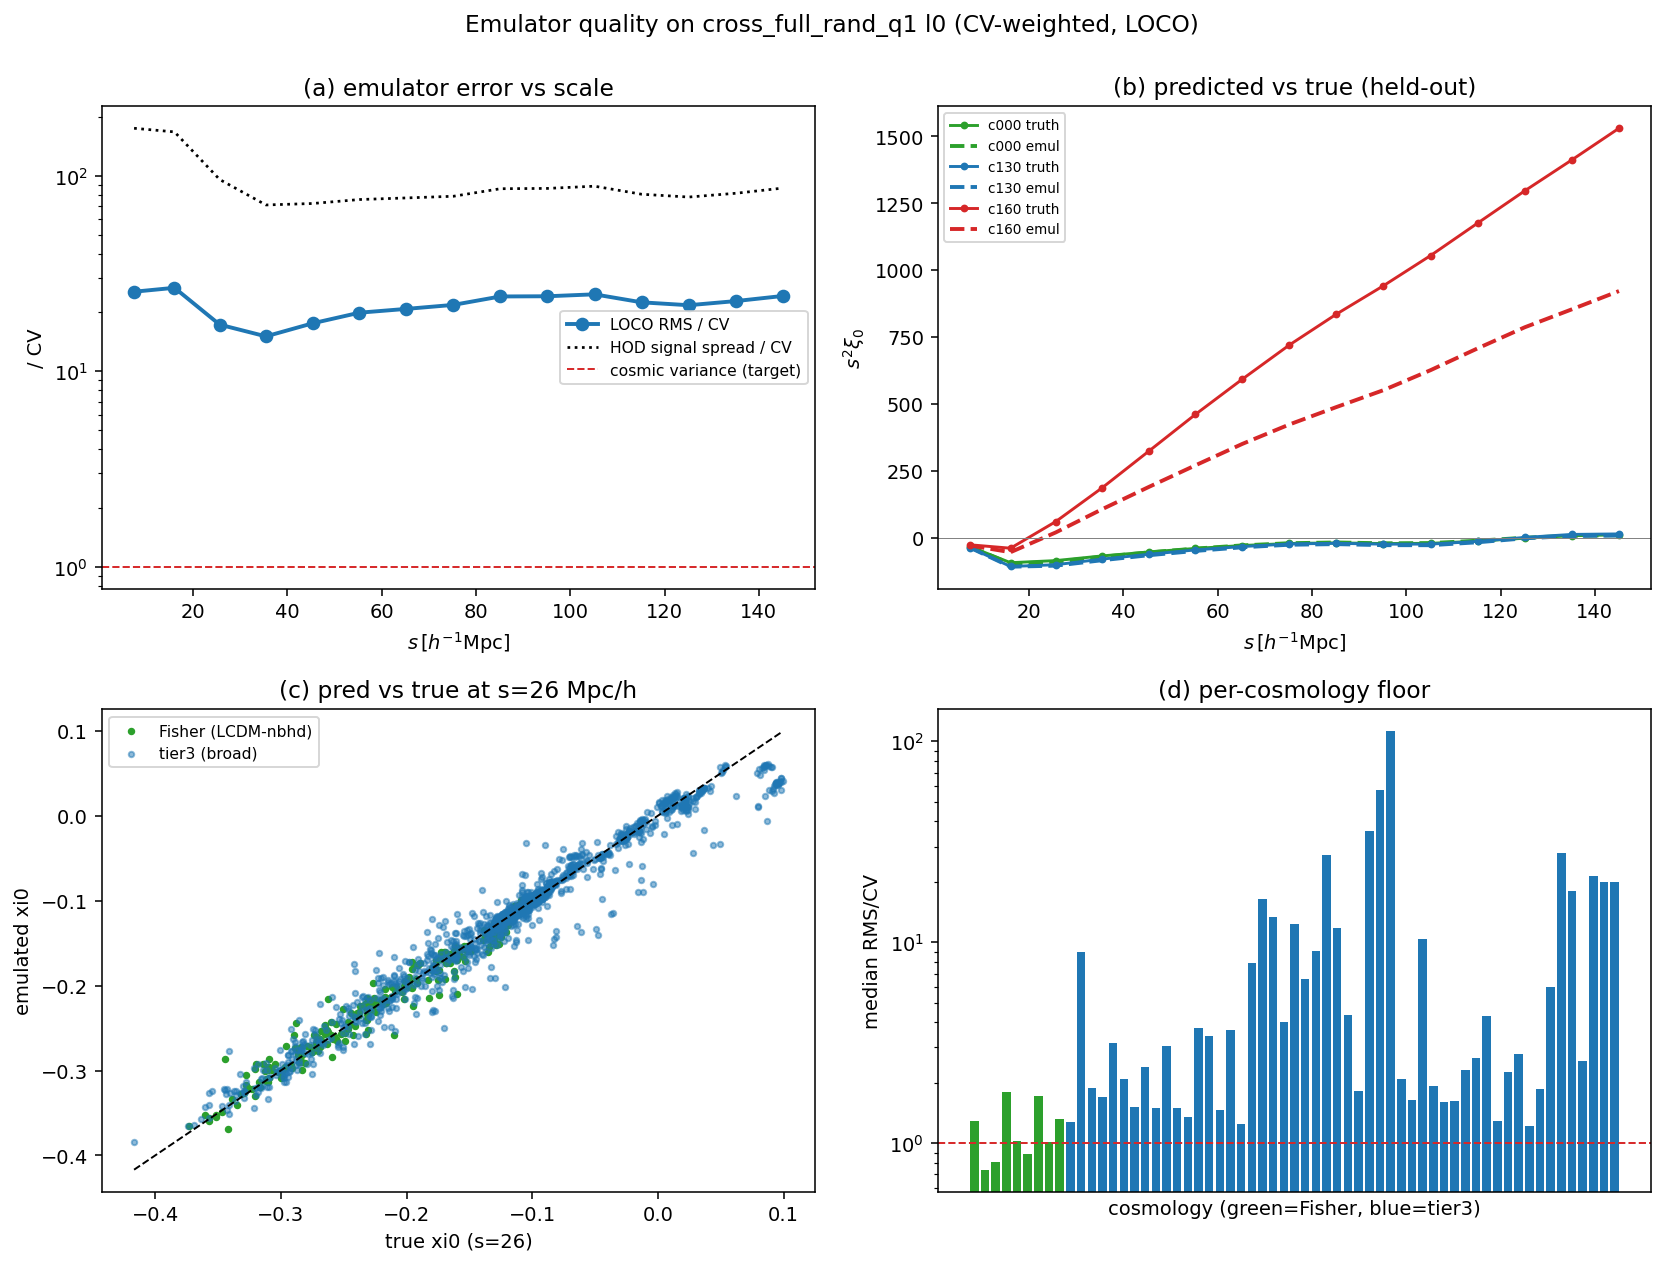
\includegraphics[width=0.49\textwidth]{leg_diagnostic_cross_full_rand_q1_l0.png}
\caption{\emph{Left:} curated value-add (synthetic) --- full 2PCF (red) vs full $+$
void-random-cross (blue); blue contours inside red ($\times$1.2--1.7). \emph{Right:}
emulator quality on the void-random-cross monopole (CV-weighted LOCO): (a) error vs
scale, (b) pred-vs-true ($c000$/$c130$ good, $c160$ edge fails), (c) pred-vs-true
scatter, (d) per-cosmology floor (Fisher $\sim$1$\times$, tier-3 scattered).}
\label{fig:curval}\label{fig:legdiag}
\end{figure}

%======================================================================
\section{Results IX: dark energy (w0, wa), and iterations are NOT the lever}
\paragraph{Recovering w0, wa.} Adding the full-2PCF quadrupole (the AP/RSD handle) we
recover three held-out tier-3 cosmologies with non-trivial dark energy
(\code{inference\_w0wa.py}; \code{c178},\code{c147},\code{c157}). $\chi^2/{\rm
dof}\!\approx\!1$ (well calibrated) and \textbf{$w_a$ is recovered within
$\sim$1.5$\sigma$} in all three; but $w_0$ and the LCDM params are biased 2--4$\sigma$.
The bias is \emph{not} the sampler --- it is the per-run emulator error at these
\emph{held-out tier-3 (extrapolation)} cosmologies ($\sim$2--4$\times$CV), exactly as
the $c000$ \emph{interpolation} recovery was unbiased. So the dark-energy bias shrinks
with \textbf{coverage}, not iterations.

\paragraph{Iterations are not the quadrupole lever (a correction).} A zero-compute test
(\code{quad\_noise\_vs\_iters.py}, Fig.~\ref{fig:quadnoise}) propagates the stored
per-iteration scatter as $\sigma_1/\sqrt{N}$: the quadrupole ASTRA-iteration noise is
\textbf{already only $\sim$0.2--0.4$\times$CV at $N=3$} (full-sample $\ell2$ $\sim$0,
since it does not depend on the quantile split), falling to $\sim$0.1$\times$ only by
$N=25$. Since the quadrupole \emph{emulator} error is $\sim$3$\times$CV, iteration noise
is $\sim$10\% of it ($\sim$1\% in variance) --- \textbf{more iterations barely move the
quadrupole $C_{\rm emu}$.} The earlier ``quads need $\sim$25 iterations'' used
noise/\emph{spread} (vs the small HOD signal), a different quantity from the
inference-relevant noise/CV. \emph{The quadrupole/dark-energy floor is coverage-limited,
not iteration-limited.}

\begin{figure}[h]\centering
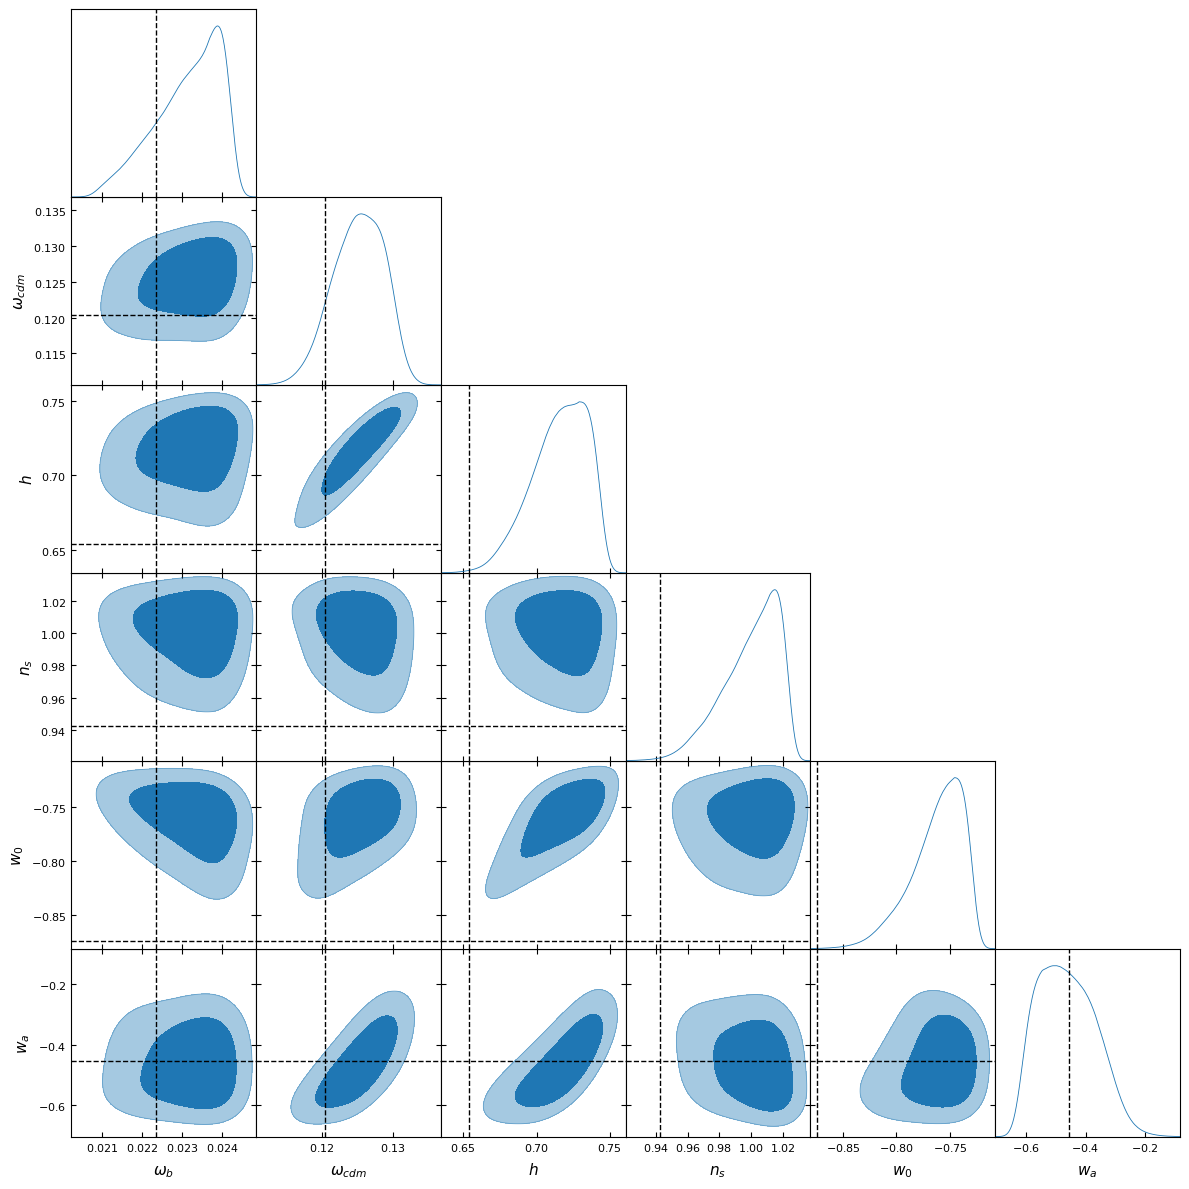
\includegraphics[width=0.49\textwidth]{inference_w0wa_c178.png}\hfill
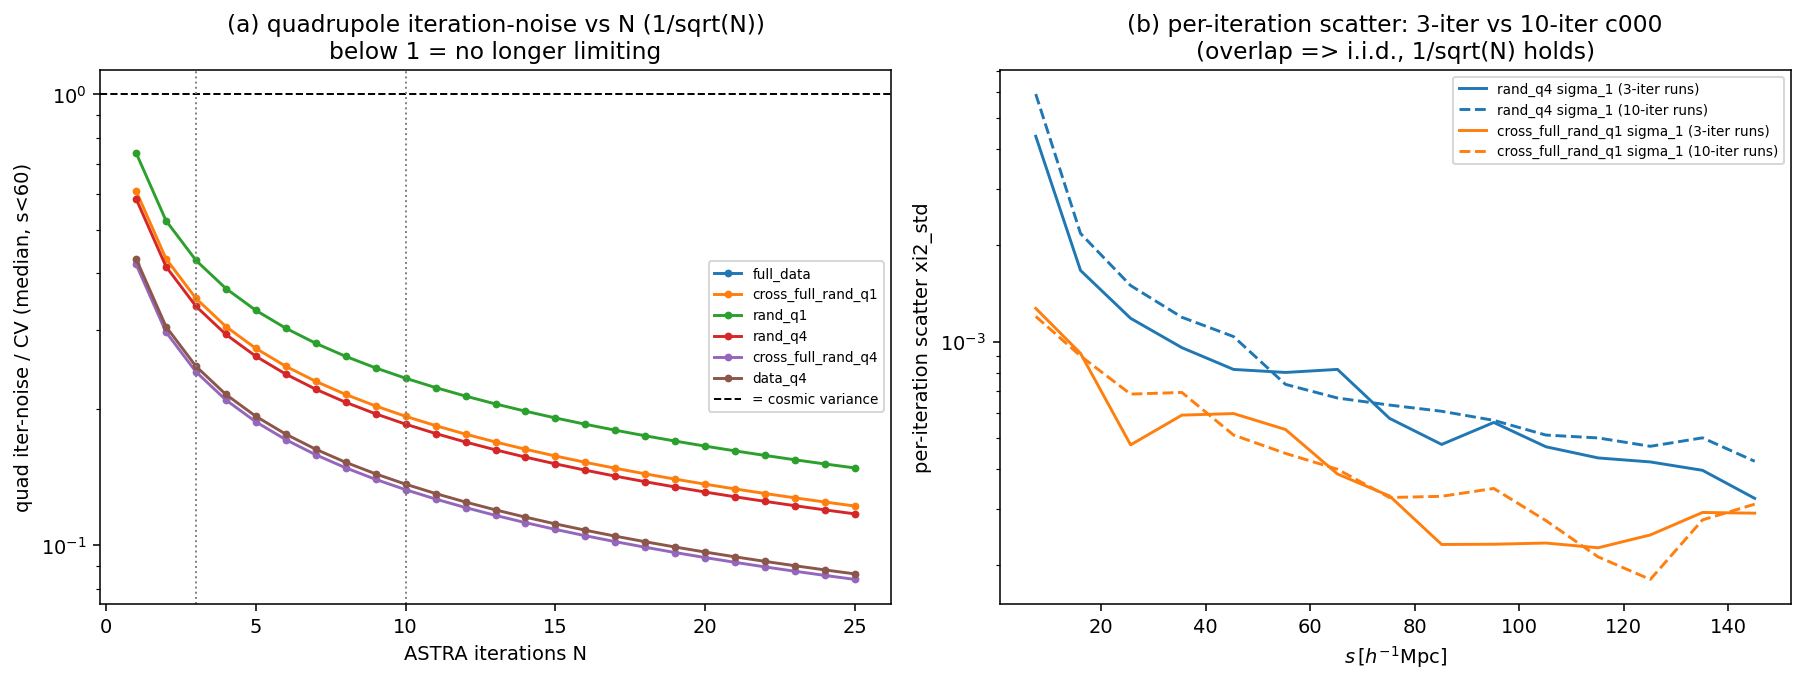
\includegraphics[width=0.49\textwidth]{quad_noise_vs_iters.png}
\caption{\emph{Left:} six-parameter recovery of \code{c178} ($w_0{=}{-}0.87$,
$w_a{=}{-}0.46$); $w_a$ recovered, $w_0$/LCDM biased (tier-3 extrapolation).
\emph{Right:} quadrupole iteration-noise/CV vs $N$ --- already below 1 at $N=3$, so
iterations are a minor lever; the per-iteration scatter from 3- vs 10-iteration
$c000$ runs overlaps, confirming the $1/\sqrt{N}$ law.}
\label{fig:quadnoise}
\end{figure}

%======================================================================
\section{Status and next steps}
\textbf{Summary.} The emulator floor is understood and is not a wall. Monopoles are
inference-grade near LCDM ($\sim$1$\times$CV) and, after the coverage run, across most
of the broad prior (tier-3 median 3.3$\times$CV, from $\sim$18$\times$). The only
remaining limiters are \emph{cosmology coverage at the 8-D hull corners}
($\to$ the denser full campaign) and \emph{quadrupole iteration noise}
($\to$ a $\geq$10-iteration run). The SUNBIRD-style inference pipeline is built and
its machinery validated on synthetic mocks; broad-prior recovery is now attempted.

\textbf{Two free wins banked since the coverage run:} (i) \textbf{CV-weighted loss}
(\S\,13) --- a $\sim$15$\times$ accuracy gain on the environment legs that tightens all
inference and partially unlocks the ASTRA value-add; (ii) \textbf{HOD marginalisation
is cheap} (\S\,14) --- only $\sim$1.0--1.8$\times$ error inflation, not the feared
2--10$\times$.

\textbf{Curated vector now.} The emulator-aware greedy (\S\,15) says a strong vector
\emph{today} is the void$\times$full cross monopole $+$ full 2PCF ($\ell0,\ell2$) $+$
void-data monopole --- notably led by an ASTRA leg, not the plain 2PCF.

\textbf{Remaining levers, now sharply targeted.} The single quantitative goal is to
drive the environment-leg $C_{\rm emu}$ \emph{well below} cosmic variance --- the
greedy shows $\sim$0.1$\times$CV (not merely $<$CV) is needed to unlock the full
$\sim$5$\times$ FoM gain; each step down converts into ASTRA value-add.

\textbf{Campaign design, corrected (\S\,17).} The dominant lever is \emph{cosmology
coverage} --- it sets the per-run extrapolation error that biases tier-3/dark-energy
recoveries and inflates the environment-leg $C_{\rm emu}$. Iterations are a
\emph{minor} lever (quadrupole iteration noise is already $\lesssim$0.4$\times$CV at
$N=3$): $N\!\approx\!6$--10 is plenty, \emph{not} 25. HODs are saturated by $\sim$30.
So spend the budget on \textbf{cosmologies first} (densify the c130--c181 hull,
especially the corners), \textbf{$\sim$10 iterations}, and \textbf{$\sim$30--40 HODs} ---
not the original 120-HOD/high-iteration plan. Routes: (1) the full \code{c130}--\code{c181}$\times$100$\times$10 campaign
(free on overrun) for corner coverage \emph{and} the iterations that kill the
random/quadrupole label noise; (2) a neighbourhood-matched $C_{\rm emu}$ (broad-prior
errors are currently inflated $\sim$16$\times$ by distant hull-corner cosmologies);
(3) an external pre-populated mock suite for an honest covariance and independent-phase
recovery mocks (removes the real-mock bias of \S\,14).

\end{document}
